% Options for packages loaded elsewhere
\PassOptionsToPackage{unicode}{hyperref}
\PassOptionsToPackage{hyphens}{url}
%
\documentclass[
  ignorenonframetext,
]{beamer}
\usepackage{pgfpages}
\setbeamertemplate{caption}[numbered]
\setbeamertemplate{caption label separator}{: }
\setbeamercolor{caption name}{fg=normal text.fg}
\beamertemplatenavigationsymbolsempty
% Prevent slide breaks in the middle of a paragraph
\widowpenalties 1 10000
\raggedbottom
\setbeamertemplate{part page}{
  \centering
  \begin{beamercolorbox}[sep=16pt,center]{part title}
    \usebeamerfont{part title}\insertpart\par
  \end{beamercolorbox}
}
\setbeamertemplate{section page}{
  \centering
  \begin{beamercolorbox}[sep=12pt,center]{section title}
    \usebeamerfont{section title}\insertsection\par
  \end{beamercolorbox}
}
\setbeamertemplate{subsection page}{
  \centering
  \begin{beamercolorbox}[sep=8pt,center]{subsection title}
    \usebeamerfont{subsection title}\insertsubsection\par
  \end{beamercolorbox}
}
\AtBeginPart{
  \frame{\partpage}
}
\AtBeginSection{
  \ifbibliography
  \else
    \frame{\sectionpage}
  \fi
}
\AtBeginSubsection{
  \frame{\subsectionpage}
}
\usepackage{amsmath,amssymb}
\usepackage{iftex}
\ifPDFTeX
  \usepackage[T1]{fontenc}
  \usepackage[utf8]{inputenc}
  \usepackage{textcomp} % provide euro and other symbols
\else % if luatex or xetex
  \usepackage{unicode-math} % this also loads fontspec
  \defaultfontfeatures{Scale=MatchLowercase}
  \defaultfontfeatures[\rmfamily]{Ligatures=TeX,Scale=1}
\fi
\usepackage{lmodern}
\usetheme[]{Madrid}
\usefonttheme{professionalfonts}
\ifPDFTeX\else
  % xetex/luatex font selection
\fi
% Use upquote if available, for straight quotes in verbatim environments
\IfFileExists{upquote.sty}{\usepackage{upquote}}{}
\IfFileExists{microtype.sty}{% use microtype if available
  \usepackage[]{microtype}
  \UseMicrotypeSet[protrusion]{basicmath} % disable protrusion for tt fonts
}{}
\makeatletter
\@ifundefined{KOMAClassName}{% if non-KOMA class
  \IfFileExists{parskip.sty}{%
    \usepackage{parskip}
  }{% else
    \setlength{\parindent}{0pt}
    \setlength{\parskip}{6pt plus 2pt minus 1pt}}
}{% if KOMA class
  \KOMAoptions{parskip=half}}
\makeatother
\usepackage{xcolor}
\newif\ifbibliography
\usepackage{color}
\usepackage{fancyvrb}
\newcommand{\VerbBar}{|}
\newcommand{\VERB}{\Verb[commandchars=\\\{\}]}
\DefineVerbatimEnvironment{Highlighting}{Verbatim}{commandchars=\\\{\}}
% Add ',fontsize=\small' for more characters per line
\usepackage{framed}
\definecolor{shadecolor}{RGB}{248,248,248}
\newenvironment{Shaded}{\begin{snugshade}}{\end{snugshade}}
\newcommand{\AlertTok}[1]{\textcolor[rgb]{0.94,0.16,0.16}{#1}}
\newcommand{\AnnotationTok}[1]{\textcolor[rgb]{0.56,0.35,0.01}{\textbf{\textit{#1}}}}
\newcommand{\AttributeTok}[1]{\textcolor[rgb]{0.13,0.29,0.53}{#1}}
\newcommand{\BaseNTok}[1]{\textcolor[rgb]{0.00,0.00,0.81}{#1}}
\newcommand{\BuiltInTok}[1]{#1}
\newcommand{\CharTok}[1]{\textcolor[rgb]{0.31,0.60,0.02}{#1}}
\newcommand{\CommentTok}[1]{\textcolor[rgb]{0.56,0.35,0.01}{\textit{#1}}}
\newcommand{\CommentVarTok}[1]{\textcolor[rgb]{0.56,0.35,0.01}{\textbf{\textit{#1}}}}
\newcommand{\ConstantTok}[1]{\textcolor[rgb]{0.56,0.35,0.01}{#1}}
\newcommand{\ControlFlowTok}[1]{\textcolor[rgb]{0.13,0.29,0.53}{\textbf{#1}}}
\newcommand{\DataTypeTok}[1]{\textcolor[rgb]{0.13,0.29,0.53}{#1}}
\newcommand{\DecValTok}[1]{\textcolor[rgb]{0.00,0.00,0.81}{#1}}
\newcommand{\DocumentationTok}[1]{\textcolor[rgb]{0.56,0.35,0.01}{\textbf{\textit{#1}}}}
\newcommand{\ErrorTok}[1]{\textcolor[rgb]{0.64,0.00,0.00}{\textbf{#1}}}
\newcommand{\ExtensionTok}[1]{#1}
\newcommand{\FloatTok}[1]{\textcolor[rgb]{0.00,0.00,0.81}{#1}}
\newcommand{\FunctionTok}[1]{\textcolor[rgb]{0.13,0.29,0.53}{\textbf{#1}}}
\newcommand{\ImportTok}[1]{#1}
\newcommand{\InformationTok}[1]{\textcolor[rgb]{0.56,0.35,0.01}{\textbf{\textit{#1}}}}
\newcommand{\KeywordTok}[1]{\textcolor[rgb]{0.13,0.29,0.53}{\textbf{#1}}}
\newcommand{\NormalTok}[1]{#1}
\newcommand{\OperatorTok}[1]{\textcolor[rgb]{0.81,0.36,0.00}{\textbf{#1}}}
\newcommand{\OtherTok}[1]{\textcolor[rgb]{0.56,0.35,0.01}{#1}}
\newcommand{\PreprocessorTok}[1]{\textcolor[rgb]{0.56,0.35,0.01}{\textit{#1}}}
\newcommand{\RegionMarkerTok}[1]{#1}
\newcommand{\SpecialCharTok}[1]{\textcolor[rgb]{0.81,0.36,0.00}{\textbf{#1}}}
\newcommand{\SpecialStringTok}[1]{\textcolor[rgb]{0.31,0.60,0.02}{#1}}
\newcommand{\StringTok}[1]{\textcolor[rgb]{0.31,0.60,0.02}{#1}}
\newcommand{\VariableTok}[1]{\textcolor[rgb]{0.00,0.00,0.00}{#1}}
\newcommand{\VerbatimStringTok}[1]{\textcolor[rgb]{0.31,0.60,0.02}{#1}}
\newcommand{\WarningTok}[1]{\textcolor[rgb]{0.56,0.35,0.01}{\textbf{\textit{#1}}}}
\setlength{\emergencystretch}{3em} % prevent overfull lines
\providecommand{\tightlist}{%
  \setlength{\itemsep}{0pt}\setlength{\parskip}{0pt}}
\setcounter{secnumdepth}{-\maxdimen} % remove section numbering
\usepackage{amsmath}
\usepackage{amssymb}
\usepackage{graphicx}
\usepackage{booktabs}
\usepackage{tikz}
\usepackage{xcolor}
\definecolor{datablue}{RGB}{0,102,204}
\definecolor{datagreen}{RGB}{0,153,76}
\definecolor{datared}{RGB}{204,0,0}
\definecolor{dataorange}{RGB}{255,140,0}
\definecolor{datapurple}{RGB}{128,0,128}
\definecolor{datacyan}{RGB}{0,191,255}
\setbeamercolor{structure}{fg=datablue}
\setbeamertemplate{navigation symbols}{}
\setbeamertemplate{footline}[frame number]
\setbeamertemplate{frametitle}{\vspace{0.5em}\insertframetitle}
\usepackage{booktabs}
\usepackage{longtable}
\usepackage{array}
\usepackage{multirow}
\usepackage{wrapfig}
\usepackage{float}
\usepackage{colortbl}
\usepackage{pdflscape}
\usepackage{tabu}
\usepackage{threeparttable}
\usepackage{threeparttablex}
\usepackage[normalem]{ulem}
\usepackage{makecell}
\usepackage{xcolor}
\usepackage{bookmark}
\IfFileExists{xurl.sty}{\usepackage{xurl}}{} % add URL line breaks if available
\urlstyle{same}
\hypersetup{
  pdfauthor={Prof.~Asc. Endri Raco, Ph.D.},
  hidelinks,
  pdfcreator={LaTeX via pandoc}}

\title{\textbf{Homophily Analysis and}\\
\textbf{Network-Based Prediction}}
\subtitle{Predictive Analytics Using Networked Data in R}
\author{Prof.~Asc. Endri Raco, Ph.D.}
\date{November 2025}
\institute{Department of Mathematical Engineering\\
Polytechnic University of Tirana}

\begin{document}
\frame{\titlepage}

\section{Introduction}\label{introduction}

\begin{frame}{Motivation: Social Networks and Predictive Analytics}
\phantomsection\label{motivation-social-networks-and-predictive-analytics}
\begin{block}{Real-World Applications}
\begin{itemize}
  \item \textbf{Age prediction}: Customer demographics
  \item \textbf{Gender inference}: Targeted marketing
  \item \textbf{Fraud detection}: Transaction network analysis
  \item \textbf{Churn prediction}: Customer defection
\end{itemize}
\end{block}

\vspace{1em}

\begin{exampleblock}{The Network Advantage}
Companies predict churn using:
\begin{enumerate}
  \item Traditional machine learning techniques
  \item \textcolor{datagreen}{\textbf{Social networks}} (relational data)
\end{enumerate}
\end{exampleblock}
\end{frame}

\begin{frame}{Course Overview}
\phantomsection\label{course-overview}
\begin{block}{Module 1: Labeled Social Networks}
\begin{itemize}
  \item Construct networks from data
  \item Label nodes with attributes
  \item Apply network learning techniques
\end{itemize}
\end{block}

\begin{block}{Module 2: Homophily Analysis}
\begin{itemize}
  \item Measure relational dependency
  \item Understand influence patterns
  \item Quantify heterophilicity and dyadicity
\end{itemize}
\end{block}
\end{frame}

\begin{frame}{Course Overview (continued)}
\phantomsection\label{course-overview-continued}
\begin{block}{Module 3: Network Featurization}
\begin{itemize}
  \item Compute node-level features
  \item Extract structural properties
  \item Create predictive variables
\end{itemize}
\end{block}

\begin{block}{Module 4: Predictive Modeling}
\begin{itemize}
  \item Transform networks into flat datasets
  \item Build prediction models
  \item Deploy churn prediction systems
\end{itemize}
\end{block}
\end{frame}

\section{Building Networks}\label{building-networks}

\begin{frame}{Network Structure Example}
\phantomsection\label{network-structure-example}
\begin{center}
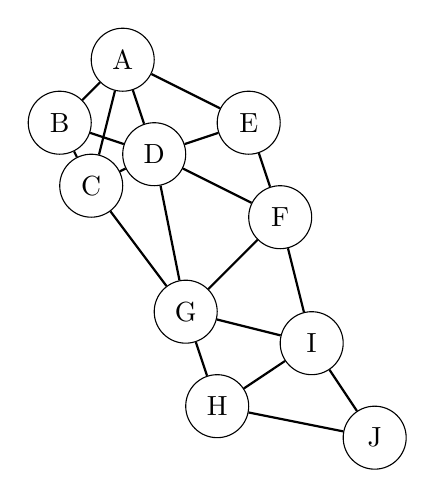
\begin{tikzpicture}[scale=0.8]
  % Draw nodes
  \node[circle, draw, fill=white, minimum size=0.8cm] (A) at (2, 4) {A};
  \node[circle, draw, fill=white, minimum size=0.8cm] (B) at (1, 3) {B};
  \node[circle, draw, fill=white, minimum size=0.8cm] (C) at (1.5, 2) {C};
  \node[circle, draw, fill=white, minimum size=0.8cm] (D) at (2.5, 2.5) {D};
  \node[circle, draw, fill=white, minimum size=0.8cm] (E) at (4, 3) {E};
  \node[circle, draw, fill=white, minimum size=0.8cm] (F) at (4.5, 1.5) {F};
  \node[circle, draw, fill=white, minimum size=0.8cm] (G) at (3, 0) {G};
  \node[circle, draw, fill=white, minimum size=0.8cm] (H) at (3.5, -1.5) {H};
  \node[circle, draw, fill=white, minimum size=0.8cm] (I) at (5, -0.5) {I};
  \node[circle, draw, fill=white, minimum size=0.8cm] (J) at (6, -2) {J};
  
  % Draw edges
  \draw[thick] (A) -- (B);
  \draw[thick] (A) -- (C);
  \draw[thick] (A) -- (D);
  \draw[thick] (A) -- (E);
  \draw[thick] (B) -- (C);
  \draw[thick] (B) -- (D);
  \draw[thick] (C) -- (D);
  \draw[thick] (C) -- (G);
  \draw[thick] (D) -- (E);
  \draw[thick] (D) -- (F);
  \draw[thick] (D) -- (G);
  \draw[thick] (E) -- (F);
  \draw[thick] (F) -- (G);
  \draw[thick] (F) -- (I);
  \draw[thick] (G) -- (I);
  \draw[thick] (G) -- (H);
  \draw[thick] (H) -- (I);
  \draw[thick] (H) -- (J);
  \draw[thick] (I) -- (J);
\end{tikzpicture}
\end{center}

\begin{block}{Network Components}
\textbf{Nodes}: Individuals (A, B, C, ...) \\
\textbf{Edges}: Relationships/collaborations \\
\textbf{Attributes}: Technology preference (R, Python, ?)
\end{block}
\end{frame}

\begin{frame}[fragile]{Creating Networks in R}
\phantomsection\label{creating-networks-in-r}
\begin{Shaded}
\begin{Highlighting}[]
\FunctionTok{library}\NormalTok{(igraph)}

\CommentTok{\# Define edges (relationships)}
\NormalTok{DataScienceNetwork }\OtherTok{\textless{}{-}} \FunctionTok{data.frame}\NormalTok{(}
  \AttributeTok{from =} \FunctionTok{c}\NormalTok{(}\StringTok{\textquotesingle{}A\textquotesingle{}}\NormalTok{,}\StringTok{\textquotesingle{}A\textquotesingle{}}\NormalTok{,}\StringTok{\textquotesingle{}A\textquotesingle{}}\NormalTok{,}\StringTok{\textquotesingle{}A\textquotesingle{}}\NormalTok{,}\StringTok{\textquotesingle{}B\textquotesingle{}}\NormalTok{,}\StringTok{\textquotesingle{}B\textquotesingle{}}\NormalTok{,}\StringTok{\textquotesingle{}C\textquotesingle{}}\NormalTok{,}\StringTok{\textquotesingle{}C\textquotesingle{}}\NormalTok{,}
           \StringTok{\textquotesingle{}D\textquotesingle{}}\NormalTok{,}\StringTok{\textquotesingle{}D\textquotesingle{}}\NormalTok{,}\StringTok{\textquotesingle{}D\textquotesingle{}}\NormalTok{,}\StringTok{\textquotesingle{}E\textquotesingle{}}\NormalTok{,}\StringTok{\textquotesingle{}F\textquotesingle{}}\NormalTok{,}\StringTok{\textquotesingle{}F\textquotesingle{}}\NormalTok{,}\StringTok{\textquotesingle{}G\textquotesingle{}}\NormalTok{,}\StringTok{\textquotesingle{}G\textquotesingle{}}\NormalTok{,}
           \StringTok{\textquotesingle{}H\textquotesingle{}}\NormalTok{,}\StringTok{\textquotesingle{}H\textquotesingle{}}\NormalTok{,}\StringTok{\textquotesingle{}I\textquotesingle{}}\NormalTok{),}
  \AttributeTok{to =} \FunctionTok{c}\NormalTok{(}\StringTok{\textquotesingle{}B\textquotesingle{}}\NormalTok{,}\StringTok{\textquotesingle{}C\textquotesingle{}}\NormalTok{,}\StringTok{\textquotesingle{}D\textquotesingle{}}\NormalTok{,}\StringTok{\textquotesingle{}E\textquotesingle{}}\NormalTok{,}\StringTok{\textquotesingle{}C\textquotesingle{}}\NormalTok{,}\StringTok{\textquotesingle{}D\textquotesingle{}}\NormalTok{,}\StringTok{\textquotesingle{}D\textquotesingle{}}\NormalTok{,}\StringTok{\textquotesingle{}G\textquotesingle{}}\NormalTok{,}
         \StringTok{\textquotesingle{}E\textquotesingle{}}\NormalTok{,}\StringTok{\textquotesingle{}F\textquotesingle{}}\NormalTok{,}\StringTok{\textquotesingle{}G\textquotesingle{}}\NormalTok{,}\StringTok{\textquotesingle{}F\textquotesingle{}}\NormalTok{,}\StringTok{\textquotesingle{}G\textquotesingle{}}\NormalTok{,}\StringTok{\textquotesingle{}I\textquotesingle{}}\NormalTok{,}\StringTok{\textquotesingle{}I\textquotesingle{}}\NormalTok{,}\StringTok{\textquotesingle{}H\textquotesingle{}}\NormalTok{,}
         \StringTok{\textquotesingle{}I\textquotesingle{}}\NormalTok{,}\StringTok{\textquotesingle{}J\textquotesingle{}}\NormalTok{,}\StringTok{\textquotesingle{}J\textquotesingle{}}\NormalTok{)}
\NormalTok{)}

\CommentTok{\# Create graph object}
\NormalTok{g }\OtherTok{\textless{}{-}} \FunctionTok{graph\_from\_data\_frame}\NormalTok{(DataScienceNetwork, }
                           \AttributeTok{directed =} \ConstantTok{FALSE}\NormalTok{)}
\end{Highlighting}
\end{Shaded}

\begin{alertblock}{Key Concept}
\texttt{graph\_from\_data\_frame()} creates an undirected graph where each row defines a connection between two nodes.
\end{alertblock}
\end{frame}

\begin{frame}[fragile]{Visualizing Networks (1/2)}
\phantomsection\label{visualizing-networks-12}
\begin{Shaded}
\begin{Highlighting}[]
\CommentTok{\# Define node positions for clean layout}
\NormalTok{pos }\OtherTok{\textless{}{-}} \FunctionTok{cbind}\NormalTok{(}
  \FunctionTok{c}\NormalTok{(}\DecValTok{2}\NormalTok{, }\DecValTok{1}\NormalTok{, }\FloatTok{1.5}\NormalTok{, }\FloatTok{2.5}\NormalTok{, }\DecValTok{4}\NormalTok{, }\FloatTok{4.5}\NormalTok{, }\DecValTok{3}\NormalTok{, }\FloatTok{3.5}\NormalTok{, }\DecValTok{5}\NormalTok{, }\DecValTok{6}\NormalTok{),}
  \FunctionTok{c}\NormalTok{(}\FloatTok{10.5}\NormalTok{, }\FloatTok{9.5}\NormalTok{, }\DecValTok{8}\NormalTok{, }\FloatTok{8.5}\NormalTok{, }\DecValTok{9}\NormalTok{, }\FloatTok{7.5}\NormalTok{, }\DecValTok{6}\NormalTok{, }\FloatTok{4.5}\NormalTok{, }\FloatTok{5.5}\NormalTok{, }\DecValTok{4}\NormalTok{)}
\NormalTok{)}

\CommentTok{\# Create visualization}
\FunctionTok{plot.igraph}\NormalTok{(g, }
            \AttributeTok{edge.label =} \ConstantTok{NA}\NormalTok{,}
            \AttributeTok{edge.color =} \StringTok{\textquotesingle{}black\textquotesingle{}}\NormalTok{,}
            \AttributeTok{layout =}\NormalTok{ pos,}
            \AttributeTok{vertex.label =} \FunctionTok{V}\NormalTok{(g)}\SpecialCharTok{$}\NormalTok{name,}
            \AttributeTok{vertex.color =} \StringTok{\textquotesingle{}white\textquotesingle{}}\NormalTok{,}
            \AttributeTok{vertex.label.color =} \StringTok{\textquotesingle{}black\textquotesingle{}}\NormalTok{,}
            \AttributeTok{vertex.size =} \DecValTok{25}\NormalTok{)}
\end{Highlighting}
\end{Shaded}
\end{frame}

\begin{frame}{Visualizing Networks (2/2)}
\phantomsection\label{visualizing-networks-22}
\begin{block}{Visualization Parameters}
\begin{description}
  \item[\texttt{layout}] Node positioning (x, y coordinates)
  \item[\texttt{vertex.*}] Node styling (color, size, labels)
  \item[\texttt{edge.*}] Connection styling (color, width, labels)
\end{description}
\end{block}

\vspace{1em}

\begin{exampleblock}{Pro Tip}
Use \texttt{layout\_nicely()} for automatic positioning, or define custom positions for publication-quality figures.
\end{exampleblock}
\end{frame}

\begin{frame}[fragile]{Adding Node Attributes}
\phantomsection\label{adding-node-attributes}
\begin{Shaded}
\begin{Highlighting}[]
\CommentTok{\# Assign technology preference to each node}
\FunctionTok{V}\NormalTok{(g)}\SpecialCharTok{$}\NormalTok{technology }\OtherTok{\textless{}{-}} \FunctionTok{c}\NormalTok{(}\StringTok{\textquotesingle{}R\textquotesingle{}}\NormalTok{,}\StringTok{\textquotesingle{}R\textquotesingle{}}\NormalTok{,}\StringTok{\textquotesingle{}?\textquotesingle{}}\NormalTok{,}\StringTok{\textquotesingle{}R\textquotesingle{}}\NormalTok{,}\StringTok{\textquotesingle{}R\textquotesingle{}}\NormalTok{,}
                     \StringTok{\textquotesingle{}R\textquotesingle{}}\NormalTok{,}\StringTok{\textquotesingle{}P\textquotesingle{}}\NormalTok{,}\StringTok{\textquotesingle{}P\textquotesingle{}}\NormalTok{,}\StringTok{\textquotesingle{}P\textquotesingle{}}\NormalTok{,}\StringTok{\textquotesingle{}P\textquotesingle{}}\NormalTok{)}

\CommentTok{\# Map preferences to colors}
\FunctionTok{V}\NormalTok{(g)}\SpecialCharTok{$}\NormalTok{color }\OtherTok{\textless{}{-}} \FunctionTok{V}\NormalTok{(g)}\SpecialCharTok{$}\NormalTok{technology}
\FunctionTok{V}\NormalTok{(g)}\SpecialCharTok{$}\NormalTok{color }\OtherTok{\textless{}{-}} \FunctionTok{gsub}\NormalTok{(}\StringTok{\textquotesingle{}R\textquotesingle{}}\NormalTok{, }\StringTok{"blue3"}\NormalTok{, }\FunctionTok{V}\NormalTok{(g)}\SpecialCharTok{$}\NormalTok{color)}
\FunctionTok{V}\NormalTok{(g)}\SpecialCharTok{$}\NormalTok{color }\OtherTok{\textless{}{-}} \FunctionTok{gsub}\NormalTok{(}\StringTok{\textquotesingle{}P\textquotesingle{}}\NormalTok{, }\StringTok{"green4"}\NormalTok{, }\FunctionTok{V}\NormalTok{(g)}\SpecialCharTok{$}\NormalTok{color)}
\FunctionTok{V}\NormalTok{(g)}\SpecialCharTok{$}\NormalTok{color }\OtherTok{\textless{}{-}} \FunctionTok{gsub}\NormalTok{(}\StringTok{\textquotesingle{}?\textquotesingle{}}\NormalTok{, }\StringTok{"gray"}\NormalTok{, }\FunctionTok{V}\NormalTok{(g)}\SpecialCharTok{$}\NormalTok{color)}
\end{Highlighting}
\end{Shaded}

\begin{block}{Color Scheme}
\textcolor{blue}{\textbf{Blue}}: R users \quad
\textcolor{green}{\textbf{Green}}: Python users \quad
\textcolor{gray}{\textbf{Gray}}: Unknown
\end{block}

\textbf{Result:} A labeled network ready for analysis!
\end{frame}

\section{Labeled Networks and Network
Learning}\label{labeled-networks-and-network-learning}

\begin{frame}{The Churn Prediction Problem}
\phantomsection\label{the-churn-prediction-problem}
\begin{columns}[T]
\begin{column}{0.48\textwidth}
\textbf{Customer Data:}
\begin{center}
\begin{tabular}{rr}
\toprule
ID & Churn \\
\midrule
1 & 0 \\
393 & 0 \\
2573 & 0 \\
4430 & 0 \\
\rowcolor{datared!20}
926 & 1 \\
\rowcolor{datared!20}
1574 & 1 \\
\bottomrule
\end{tabular}
\end{center}
\end{column}

\begin{column}{0.48\textwidth}
\textbf{Edge List:}
\begin{center}
\begin{tabular}{rr}
\toprule
From & To \\
\midrule
1 & 393 \\
1 & 2573 \\
1 & 4430 \\
393 & 926 \\
393 & 1574 \\
\bottomrule
\end{tabular}
\end{center}
\end{column}
\end{columns}

\vspace{1em}

\begin{alertblock}{Goal}
Predict which customers will churn based on network structure
\end{alertblock}
\end{frame}

\begin{frame}{Network Representation of Churn}
\phantomsection\label{network-representation-of-churn}
\begin{center}
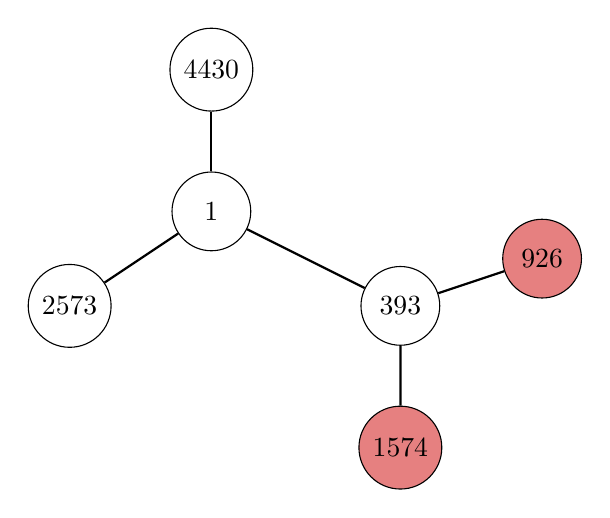
\begin{tikzpicture}[scale=1.2]
  % Nodes
  \node[circle, draw, fill=white, minimum size=1cm] (1) at (0, 2) {1};
  \node[circle, draw, fill=white, minimum size=1cm] (393) at (2, 1) {393};
  \node[circle, draw, fill=white, minimum size=1cm] (2573) at (-1.5, 1) {2573};
  \node[circle, draw, fill=white, minimum size=1cm] (4430) at (0, 3.5) {4430};
  \node[circle, draw, fill=datared!50, minimum size=1cm] (926) at (3.5, 1.5) {926};
  \node[circle, draw, fill=datared!50, minimum size=1cm] (1574) at (2, -0.5) {1574};
  
  % Edges
  \draw[thick] (1) -- (393);
  \draw[thick] (1) -- (2573);
  \draw[thick] (1) -- (4430);
  \draw[thick] (393) -- (926);
  \draw[thick] (393) -- (1574);
\end{tikzpicture}
\end{center}

\begin{block}{Key Observations}
\begin{itemize}
  \item Customer 1: Connected to 3 non-churners
  \item Customer 393: Connected to 2 churners!
  \item \textcolor{datared}{\textbf{Network structure matters}}
\end{itemize}
\end{block}
\end{frame}

\begin{frame}{The Relational Neighbor Classifier (1/2)}
\phantomsection\label{the-relational-neighbor-classifier-12}
\begin{block}{Core Principle: Homophily}
\textbf{"Birds of a feather flock together"}

Connected individuals tend to be similar in behavior and attributes.
\end{block}

\vspace{1em}

\begin{exampleblock}{Algorithm Logic}
For unknown node C (Cecelia with technology = ?):
\begin{enumerate}
  \item \textbf{Identify neighbors}: A, B, D, G
  \item \textbf{Count preferences}:
  \begin{itemize}
    \item R users: A, B, D → 3 neighbors (75\%)
    \item Python users: G → 1 neighbor (25\%)
  \end{itemize}
  \item \textbf{Predict}: Cecelia likely prefers R
\end{enumerate}
\end{exampleblock}
\end{frame}

\begin{frame}[fragile]{The Relational Neighbor Classifier (2/2)}
\phantomsection\label{the-relational-neighbor-classifier-22}
\begin{Shaded}
\begin{Highlighting}[]
\CommentTok{\# Count R{-}preferring neighbors per node}
\NormalTok{rNeighbors }\OtherTok{\textless{}{-}} \FunctionTok{c}\NormalTok{(}\DecValTok{4}\NormalTok{, }\DecValTok{3}\NormalTok{, }\DecValTok{3}\NormalTok{, }\DecValTok{5}\NormalTok{, }\DecValTok{3}\NormalTok{, }\DecValTok{2}\NormalTok{, }\DecValTok{3}\NormalTok{, }\DecValTok{0}\NormalTok{, }\DecValTok{1}\NormalTok{, }\DecValTok{0}\NormalTok{)}

\CommentTok{\# Count Python{-}preferring neighbors}
\NormalTok{pNeighbors }\OtherTok{\textless{}{-}} \FunctionTok{c}\NormalTok{(}\DecValTok{0}\NormalTok{, }\DecValTok{0}\NormalTok{, }\DecValTok{1}\NormalTok{, }\DecValTok{1}\NormalTok{, }\DecValTok{0}\NormalTok{, }\DecValTok{2}\NormalTok{, }\DecValTok{2}\NormalTok{, }\DecValTok{3}\NormalTok{, }\DecValTok{3}\NormalTok{, }\DecValTok{2}\NormalTok{)}

\CommentTok{\# Calculate probability of preferring R}
\NormalTok{rRelationalNeighbor }\OtherTok{\textless{}{-}}\NormalTok{ rNeighbors }\SpecialCharTok{/} 
\NormalTok{                       (rNeighbors }\SpecialCharTok{+}\NormalTok{ pNeighbors)}

\FunctionTok{print}\NormalTok{(rRelationalNeighbor)}
\end{Highlighting}
\end{Shaded}

\begin{alertblock}{Output}
\texttt{[1] 1.00 1.00 0.75 0.83 1.00 0.50 0.60 0.00 0.25 0.00}
\end{alertblock}

Node C (index 3) has 0.75 probability of preferring R
\end{frame}

\begin{frame}{Applying RNC to Churn Prediction}
\phantomsection\label{applying-rnc-to-churn-prediction}
\begin{block}{Step-by-Step Application}
\begin{enumerate}
  \item For each customer with unknown churn status
  \item Count neighbors who churned
  \item Count neighbors who stayed
  \item Calculate: $P(\text{churn}) = \frac{\text{\# churned neighbors}}{\text{\# total neighbors}}$
  \item Predict churn if $P(\text{churn}) > 0.5$
\end{enumerate}
\end{block}

\vspace{1em}

\begin{exampleblock}{Example: Customer 393}
\begin{itemize}
  \item Churned neighbors: 926, 1574 → 2
  \item Non-churned neighbors: 1 → 1
  \item $P(\text{churn}) = \frac{2}{3} = 0.67$ → \textcolor{datared}{\textbf{Predict: CHURN}}
\end{itemize}
\end{exampleblock}
\end{frame}

\begin{frame}[fragile]{RNC Implementation in R}
\phantomsection\label{rnc-implementation-in-r}
\begin{Shaded}
\begin{Highlighting}[]
\CommentTok{\# Function to compute RNC predictions}
\NormalTok{compute\_rnc }\OtherTok{\textless{}{-}} \ControlFlowTok{function}\NormalTok{(graph, node\_labels) \{}
\NormalTok{  predictions }\OtherTok{\textless{}{-}} \FunctionTok{numeric}\NormalTok{(}\FunctionTok{vcount}\NormalTok{(graph))}
  
  \ControlFlowTok{for}\NormalTok{ (i }\ControlFlowTok{in} \DecValTok{1}\SpecialCharTok{:}\FunctionTok{vcount}\NormalTok{(graph)) \{}
    \CommentTok{\# Get neighbors}
\NormalTok{    neighbors }\OtherTok{\textless{}{-}} \FunctionTok{neighbors}\NormalTok{(graph, i)}
    
    \ControlFlowTok{if}\NormalTok{ (}\FunctionTok{length}\NormalTok{(neighbors) }\SpecialCharTok{==} \DecValTok{0}\NormalTok{) \{}
\NormalTok{      predictions[i] }\OtherTok{\textless{}{-}} \ConstantTok{NA}  \CommentTok{\# Isolated node}
      \ControlFlowTok{next}
\NormalTok{    \}}
    
    \CommentTok{\# Count churned neighbors}
\NormalTok{    churned\_count }\OtherTok{\textless{}{-}} \FunctionTok{sum}\NormalTok{(node\_labels[neighbors] }\SpecialCharTok{==} \DecValTok{1}\NormalTok{)}
\NormalTok{    total\_count }\OtherTok{\textless{}{-}} \FunctionTok{length}\NormalTok{(neighbors)}
    
    \CommentTok{\# Calculate probability}
\NormalTok{    predictions[i] }\OtherTok{\textless{}{-}}\NormalTok{ churned\_count }\SpecialCharTok{/}\NormalTok{ total\_count}
\NormalTok{  \}}
  
  \FunctionTok{return}\NormalTok{(predictions)}
\NormalTok{\}}
\end{Highlighting}
\end{Shaded}
\end{frame}

\begin{frame}{Visualizing Predictions}
\phantomsection\label{visualizing-predictions}
\begin{center}
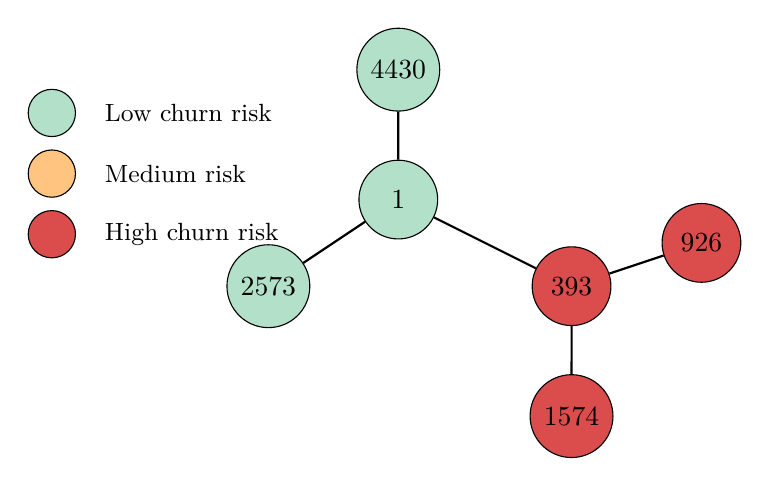
\begin{tikzpicture}[scale=1.1]
  % Legend
  \node[circle, draw, fill=datagreen!30, minimum size=0.6cm] at (-2, 3) {};
  \node[right] at (-1.5, 3) {\small Low churn risk};
  \node[circle, draw, fill=dataorange!50, minimum size=0.6cm] at (-2, 2.3) {};
  \node[right] at (-1.5, 2.3) {\small Medium risk};
  \node[circle, draw, fill=datared!70, minimum size=0.6cm] at (-2, 1.6) {};
  \node[right] at (-1.5, 1.6) {\small High churn risk};
  
  % Network with color-coded predictions
  \node[circle, draw, fill=datagreen!30, minimum size=1cm] (1) at (2, 2) {1};
  \node[circle, draw, fill=datared!70, minimum size=1cm] (393) at (4, 1) {393};
  \node[circle, draw, fill=datagreen!30, minimum size=1cm] (2573) at (0.5, 1) {2573};
  \node[circle, draw, fill=datagreen!30, minimum size=1cm] (4430) at (2, 3.5) {4430};
  \node[circle, draw, fill=datared!70, minimum size=1cm] (926) at (5.5, 1.5) {926};
  \node[circle, draw, fill=datared!70, minimum size=1cm] (1574) at (4, -0.5) {1574};
  
  \draw[thick] (1) -- (393);
  \draw[thick] (1) -- (2573);
  \draw[thick] (1) -- (4430);
  \draw[thick] (393) -- (926);
  \draw[thick] (393) -- (1574);
\end{tikzpicture}
\end{center}

Customer 393 surrounded by churners → High risk!
\end{frame}

\section{Challenges in Network
Learning}\label{challenges-in-network-learning}

\begin{frame}[fragile]{Challenge 1: Splitting Network Data}
\phantomsection\label{challenge-1-splitting-network-data}
\begin{alertblock}{Problem}
Cannot randomly split networked data like traditional datasets!
\end{alertblock}

\begin{Shaded}
\begin{Highlighting}[]
\CommentTok{\# WRONG: Random sampling breaks network structure}
\FunctionTok{set.seed}\NormalTok{(}\DecValTok{1001}\NormalTok{)}
\NormalTok{sample\_vertices }\OtherTok{\textless{}{-}} \FunctionTok{sample}\NormalTok{(}\DecValTok{1}\SpecialCharTok{:}\DecValTok{10}\NormalTok{, }\DecValTok{6}\NormalTok{, }\AttributeTok{replace =} \ConstantTok{FALSE}\NormalTok{)}
\NormalTok{train\_graph }\OtherTok{\textless{}{-}} \FunctionTok{induced\_subgraph}\NormalTok{(g, }\FunctionTok{V}\NormalTok{(g)[sample\_vertices])}
\NormalTok{test\_graph }\OtherTok{\textless{}{-}} \FunctionTok{induced\_subgraph}\NormalTok{(g, }\FunctionTok{V}\NormalTok{(g)[}\SpecialCharTok{{-}}\NormalTok{sample\_vertices])}
\end{Highlighting}
\end{Shaded}

\begin{block}{Issues with Random Split}
\begin{itemize}
  \item Breaks connections between train/test
  \item Test nodes may be isolated
  \item Cannot compute neighbor-based features
  \item Invalidates relational predictions
\end{itemize}
\end{block}
\end{frame}

\begin{frame}{Challenge 1: Visual Illustration}
\phantomsection\label{challenge-1-visual-illustration}
\begin{center}
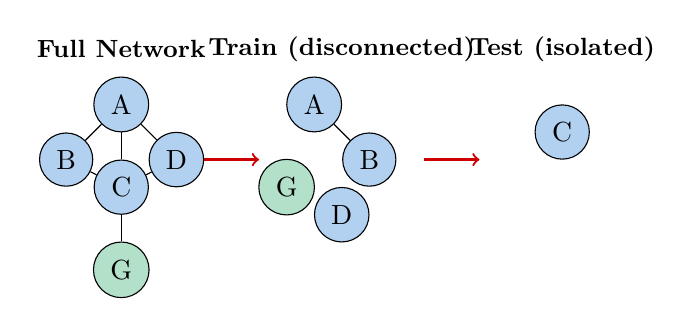
\begin{tikzpicture}[scale=0.7]
  % Original network
  \node[font=\small] at (1, 4) {\textbf{Full Network}};
  \node[circle, draw, fill=datablue!30, minimum size=0.6cm] (A) at (1, 3) {A};
  \node[circle, draw, fill=datablue!30, minimum size=0.6cm] (B) at (0, 2) {B};
  \node[circle, draw, fill=datablue!30, minimum size=0.6cm] (C) at (1, 1.5) {C};
  \node[circle, draw, fill=datablue!30, minimum size=0.6cm] (D) at (2, 2) {D};
  \node[circle, draw, fill=datagreen!30, minimum size=0.6cm] (G) at (1, 0) {G};
  \draw (A) -- (B);
  \draw (A) -- (C);
  \draw (A) -- (D);
  \draw (B) -- (C);
  \draw (C) -- (D);
  \draw (C) -- (G);
  
  % Training set
  \node[font=\small] at (5, 4) {\textbf{Train (disconnected)}};
  \node[circle, draw, fill=datablue!30, minimum size=0.6cm] (A2) at (4.5, 3) {A};
  \node[circle, draw, fill=datablue!30, minimum size=0.6cm] (B2) at (5.5, 2) {B};
  \node[circle, draw, fill=datablue!30, minimum size=0.6cm] (D2) at (5, 1) {D};
  \node[circle, draw, fill=datagreen!30, minimum size=0.6cm] (G2) at (4, 1.5) {G};
  \draw (A2) -- (B2);
  
  % Test set (isolated)
  \node[font=\small] at (9, 4) {\textbf{Test (isolated)}};
  \node[circle, draw, fill=datablue!30, minimum size=0.6cm] (C2) at (9, 2.5) {C};
  
  \draw[->, thick, datared] (2.5, 2) -- (3.5, 2);
  \draw[->, thick, datared] (6.5, 2) -- (7.5, 2);
\end{tikzpicture}
\end{center}

Node C becomes isolated → Cannot compute neighbor features!
\end{frame}

\begin{frame}{Solution: Temporal or Stratified Splits}
\phantomsection\label{solution-temporal-or-stratified-splits}
\begin{block}{Better Splitting Strategies}
\begin{enumerate}
  \item \textbf{Temporal split}:
  \begin{itemize}
    \item Use time-stamped data
    \item Train on early period, test on late period
    \item Preserves network structure
  \end{itemize}
  
  \item \textbf{Inductive split}:
  \begin{itemize}
    \item Keep full network for feature computation
    \item Split only labels (hide some during training)
    \item All nodes remain connected
  \end{itemize}
  
  \item \textbf{Cross-validation}:
  \begin{itemize}
    \item Stratified k-fold by network communities
    \item Preserve local structure in each fold
  \end{itemize}
\end{enumerate}
\end{block}
\end{frame}

\begin{frame}{Challenge 2: Non-IID Data}
\phantomsection\label{challenge-2-non-iid-data}
\begin{alertblock}{Violation of Independence Assumption}
Observations in networks are \textbf{NOT} independent and identically distributed (IID)
\end{alertblock}

\vspace{1em}

\begin{block}{Why This Matters}
\begin{itemize}
  \item Traditional ML assumes IID data
  \item Connected nodes influence each other
  \item Violates statistical assumptions
  \item Standard confidence intervals invalid
  \item P-values may be misleading
\end{itemize}
\end{block}

\vspace{1em}

\begin{exampleblock}{Consequence}
If customer A churns, their friend B becomes more likely to churn → observations are \textcolor{datared}{\textbf{dependent}}
\end{exampleblock}
\end{frame}

\begin{frame}{Challenge 2: Statistical Dependency}
\phantomsection\label{challenge-2-statistical-dependency}
\begin{center}
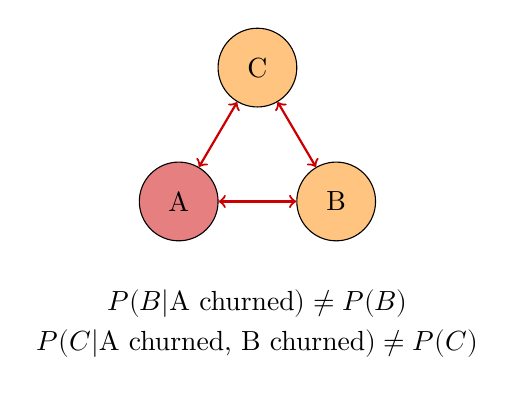
\begin{tikzpicture}[scale=1]
  % Show dependency structure
  \node[circle, draw, fill=datared!50, minimum size=1cm] (A) at (0, 0) {A};
  \node[circle, draw, fill=dataorange!50, minimum size=1cm] (B) at (2, 0) {B};
  \node[circle, draw, fill=dataorange!50, minimum size=1cm] (C) at (1, 1.7) {C};
  
  \draw[thick, <->, datared] (A) -- (B);
  \draw[thick, <->, datared] (A) -- (C);
  \draw[thick, <->, datared] (B) -- (C);
  
  \node[below] at (1, -1) {$P(B|\text{A churned}) \neq P(B)$};
  \node[below] at (1, -1.5) {$P(C|\text{A churned, B churned}) \neq P(C)$};
\end{tikzpicture}
\end{center}

\begin{block}{Implication}
Must use network-aware methods:
\begin{itemize}
  \item Network cross-validation
  \item Permutation tests respecting structure
  \item Autocorrelation-adjusted standard errors
\end{itemize}
\end{block}
\end{frame}

\begin{frame}{Challenge 3: Collective Inference}
\phantomsection\label{challenge-3-collective-inference}
\begin{block}{The Bootstrap Problem}
\textbf{Scenario}: Predict multiple unknown labels simultaneously

\textbf{Issue}: Predictions depend on each other!
\end{block}

\vspace{1em}

\begin{center}
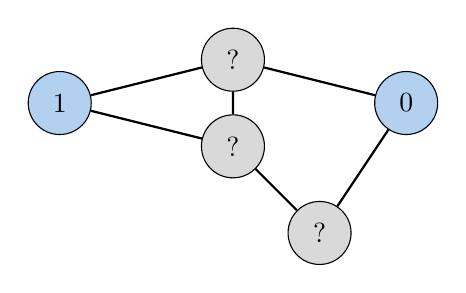
\begin{tikzpicture}[scale=1.1]
  \node[circle, draw, fill=datablue!30, minimum size=0.8cm] (known1) at (0, 2) {1};
  \node[circle, draw, fill=gray!30, minimum size=0.8cm] (unknown1) at (2, 2.5) {?};
  \node[circle, draw, fill=gray!30, minimum size=0.8cm] (unknown2) at (2, 1.5) {?};
  \node[circle, draw, fill=datablue!30, minimum size=0.8cm] (known2) at (4, 2) {0};
  \node[circle, draw, fill=gray!30, minimum size=0.8cm] (unknown3) at (3, 0.5) {?};
  
  \draw[thick] (known1) -- (unknown1);
  \draw[thick] (known1) -- (unknown2);
  \draw[thick] (unknown1) -- (unknown2);
  \draw[thick] (unknown2) -- (unknown3);
  \draw[thick] (unknown1) -- (known2);
  \draw[thick] (unknown3) -- (known2);
\end{tikzpicture}
\end{center}

Unknown nodes influence each other's predictions!
\end{frame}

\begin{frame}{Collective Inference Solution}
\phantomsection\label{collective-inference-solution}
\begin{block}{Iterative Classification Algorithm (ICA)}
\begin{enumerate}
  \item Initialize predictions for all unknown nodes
  \item \textbf{Repeat until convergence}:
  \begin{enumerate}
    \item For each unknown node:
    \begin{itemize}
      \item Compute features using current predictions
      \item Update prediction
    \end{itemize}
    \item Check if predictions changed
  \end{enumerate}
  \item Return final predictions
\end{enumerate}
\end{block}

\begin{alertblock}{Convergence}
Usually converges in 3-10 iterations
\end{alertblock}
\end{frame}

\begin{frame}{Probabilistic Relational Neighbor Classifier}
\phantomsection\label{probabilistic-relational-neighbor-classifier}
\begin{block}{Handling Uncertainty}
Use \textbf{probabilities} instead of hard labels during iteration
\end{block}

\begin{center}
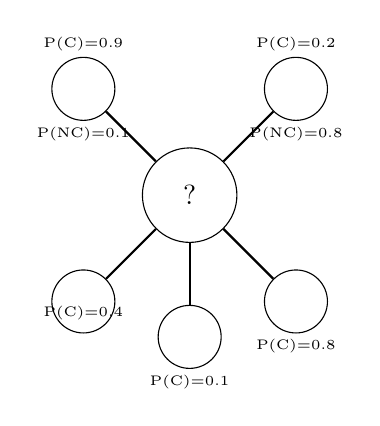
\begin{tikzpicture}[scale=0.9]
  \node[circle, draw, minimum size=1.2cm] (center) at (0, 0) {?};
  
  \node[circle, draw, minimum size=0.8cm] (n1) at (-1.5, 1.5) {};
  \node[above, font=\tiny] at (-1.5, 1.9) {P(C)=0.9};
  \node[below, font=\tiny] at (-1.5, 1.1) {P(NC)=0.1};
  
  \node[circle, draw, minimum size=0.8cm] (n2) at (1.5, 1.5) {};
  \node[above, font=\tiny] at (1.5, 1.9) {P(C)=0.2};
  \node[below, font=\tiny] at (1.5, 1.1) {P(NC)=0.8};
  
  \node[circle, draw, minimum size=0.8cm] (n3) at (-1.5, -1.5) {};
  \node[above, font=\tiny] at (-1.5, -1.9) {P(C)=0.4};
  
  \node[circle, draw, minimum size=0.8cm] (n4) at (0, -2) {};
  \node[below, font=\tiny] at (0, -2.4) {P(C)=0.1};
  
  \node[circle, draw, minimum size=0.8cm] (n5) at (1.5, -1.5) {};
  \node[below, font=\tiny] at (1.5, -1.9) {P(C)=0.8};
  
  \draw[thick] (center) -- (n1);
  \draw[thick] (center) -- (n2);
  \draw[thick] (center) -- (n3);
  \draw[thick] (center) -- (n4);
  \draw[thick] (center) -- (n5);
\end{tikzpicture}
\end{center}
\end{frame}

\begin{frame}{PRNC Calculation}
\phantomsection\label{prnc-calculation}
\begin{block}{Formula}
For unknown node $i$:
$$P(\text{churn}_i) = \frac{\sum_{j \in \mathcal{N}(i)} P(\text{churn}_j)}{|\mathcal{N}(i)|}$$

where $\mathcal{N}(i)$ = neighbors of node $i$
\end{block}

\begin{exampleblock}{Example Calculation}
Neighbors' probabilities: 0.9, 0.2, 0.4, 0.1, 0.8

$$P(\text{churn}) = \frac{0.9 + 0.2 + 0.4 + 0.1 + 0.8}{5} = \frac{2.4}{5} = 0.48$$

$$P(\text{non-churn}) = 1 - 0.48 = 0.52$$

\textbf{Prediction}: Slightly more likely to NOT churn
\end{exampleblock}
\end{frame}

\begin{frame}[fragile]{PRNC in R}
\phantomsection\label{prnc-in-r}
\begin{Shaded}
\begin{Highlighting}[]
\CommentTok{\# Probabilistic RNC computation}
\NormalTok{compute\_prnc }\OtherTok{\textless{}{-}} \ControlFlowTok{function}\NormalTok{(graph, churn\_probs) \{}
\NormalTok{  n }\OtherTok{\textless{}{-}} \FunctionTok{vcount}\NormalTok{(graph)}
\NormalTok{  new\_probs }\OtherTok{\textless{}{-}} \FunctionTok{numeric}\NormalTok{(n)}
  
  \ControlFlowTok{for}\NormalTok{ (i }\ControlFlowTok{in} \DecValTok{1}\SpecialCharTok{:}\NormalTok{n) \{}
\NormalTok{    neighbors }\OtherTok{\textless{}{-}} \FunctionTok{neighbors}\NormalTok{(graph, i)}
    
    \ControlFlowTok{if}\NormalTok{ (}\FunctionTok{length}\NormalTok{(neighbors) }\SpecialCharTok{==} \DecValTok{0}\NormalTok{) \{}
\NormalTok{      new\_probs[i] }\OtherTok{\textless{}{-}}\NormalTok{ churn\_probs[i]  }\CommentTok{\# Keep current}
\NormalTok{    \} }\ControlFlowTok{else}\NormalTok{ \{}
      \CommentTok{\# Average neighbor probabilities}
\NormalTok{      new\_probs[i] }\OtherTok{\textless{}{-}} \FunctionTok{mean}\NormalTok{(churn\_probs[neighbors])}
\NormalTok{    \}}
\NormalTok{  \}}
  
  \FunctionTok{return}\NormalTok{(new\_probs)}
\NormalTok{\}}
\end{Highlighting}
\end{Shaded}
\end{frame}

\begin{frame}[fragile]{PRNC Example}
\phantomsection\label{prnc-example}
\begin{Shaded}
\begin{Highlighting}[]
\CommentTok{\# Example: 5 neighbors with different probabilities}
\NormalTok{neighbor\_churn\_probs }\OtherTok{\textless{}{-}} \FunctionTok{c}\NormalTok{(}\FloatTok{0.9}\NormalTok{, }\FloatTok{0.2}\NormalTok{, }\FloatTok{0.1}\NormalTok{, }\FloatTok{0.4}\NormalTok{, }\FloatTok{0.8}\NormalTok{)}

\CommentTok{\# Calculate probability of churn}
\NormalTok{prob\_churn }\OtherTok{\textless{}{-}} \FunctionTok{mean}\NormalTok{(neighbor\_churn\_probs)}
\FunctionTok{print}\NormalTok{(prob\_churn)}

\CommentTok{\# Calculate probability of non{-}churn}
\NormalTok{prob\_non\_churn }\OtherTok{\textless{}{-}} \DecValTok{1} \SpecialCharTok{{-}}\NormalTok{ prob\_churn}
\FunctionTok{print}\NormalTok{(prob\_non\_churn)}
\end{Highlighting}
\end{Shaded}

\begin{block}{Output}
\texttt{[1] 0.48} \quad (churn probability)

\texttt{[1] 0.52} \quad (non-churn probability)
\end{block}

\textcolor{datagreen}{\textbf{Prediction}}: More likely to stay (52\% vs
48\%)
\end{frame}

\section{Introduction to Homophily}\label{introduction-to-homophily}

\begin{frame}{What is Homophily?}
\phantomsection\label{what-is-homophily}
\begin{block}{Definition}
\textbf{Homophily}: The tendency for similar individuals to form connections
\end{block}

\vspace{0.5em}

\textbf{``Birds of a feather flock together''}

\vspace{0.5em}

Individuals with shared characteristics are more likely to connect:

\begin{itemize}
\tightlist
\item
  Common hobbies or interests
\item
  Similar demographics
\item
  Shared technology preferences
\item
  Same geographic origin
\end{itemize}
\end{frame}

\begin{frame}{Measuring Homophily}
\phantomsection\label{measuring-homophily}
Homophily depends on two key factors:

\begin{enumerate}
  \item \textbf{Connectedness between nodes with SAME label}
  \begin{itemize}
    \item How often do similar nodes connect?
  \end{itemize}
  
  \vspace{0.5em}
  
  \item \textbf{Connectedness between nodes with OPPOSITE labels}
  \begin{itemize}
    \item How often do dissimilar nodes connect?
  \end{itemize}
\end{enumerate}

\vspace{1em}

\begin{alertblock}{Key Question}
Are labels randomly distributed, or is there structural organization?
\end{alertblock}
\end{frame}

\begin{frame}{Why Homophily Matters for Predictive Analytics}
\phantomsection\label{why-homophily-matters-for-predictive-analytics}
\begin{block}{Predictive Value}
If a network exhibits homophily:
\begin{itemize}
  \item Network structure contains information
  \item Neighbor labels help predict unknown labels
  \item Relational classifiers can be effective
\end{itemize}
\end{block}

\vspace{1em}

\begin{exampleblock}{Applications}
\begin{itemize}
  \item Customer churn prediction
  \item Fraud detection
  \item Product recommendation
  \item Technology preference inference
\end{itemize}
\end{exampleblock}
\end{frame}

\section{Building the Data Scientist
Network}\label{building-the-data-scientist-network}

\begin{frame}[fragile]{Creating Node Data}
\phantomsection\label{creating-node-data}
\begin{Shaded}
\begin{Highlighting}[]
\CommentTok{\# Define data scientists and their technology preferences}
\NormalTok{names }\OtherTok{\textless{}{-}} \FunctionTok{c}\NormalTok{(}\StringTok{\textquotesingle{}A\textquotesingle{}}\NormalTok{, }\StringTok{\textquotesingle{}B\textquotesingle{}}\NormalTok{, }\StringTok{\textquotesingle{}C\textquotesingle{}}\NormalTok{, }\StringTok{\textquotesingle{}D\textquotesingle{}}\NormalTok{, }\StringTok{\textquotesingle{}E\textquotesingle{}}\NormalTok{, }
           \StringTok{\textquotesingle{}F\textquotesingle{}}\NormalTok{, }\StringTok{\textquotesingle{}G\textquotesingle{}}\NormalTok{, }\StringTok{\textquotesingle{}H\textquotesingle{}}\NormalTok{, }\StringTok{\textquotesingle{}I\textquotesingle{}}\NormalTok{, }\StringTok{\textquotesingle{}J\textquotesingle{}}\NormalTok{)}

\NormalTok{tech }\OtherTok{\textless{}{-}} \FunctionTok{c}\NormalTok{(}\FunctionTok{rep}\NormalTok{(}\StringTok{\textquotesingle{}R\textquotesingle{}}\NormalTok{, }\DecValTok{6}\NormalTok{), }\FunctionTok{rep}\NormalTok{(}\StringTok{\textquotesingle{}P\textquotesingle{}}\NormalTok{, }\DecValTok{4}\NormalTok{))}

\CommentTok{\# Create node attribute data frame}
\NormalTok{DataScientists }\OtherTok{\textless{}{-}} \FunctionTok{data.frame}\NormalTok{(}
  \AttributeTok{name =}\NormalTok{ names,}
  \AttributeTok{technology =}\NormalTok{ tech}
\NormalTok{)}
\end{Highlighting}
\end{Shaded}

\begin{center}
\begin{tabular}{ll}
\toprule
\textbf{Node} & \textbf{Technology} \\
\midrule
A-F & R \\
G-J & Python \\
\bottomrule
\end{tabular}
\end{center}
\end{frame}

\begin{frame}[fragile]{Creating Edge Data}
\phantomsection\label{creating-edge-data}
\begin{Shaded}
\begin{Highlighting}[]
\CommentTok{\# Define collaboration connections}
\NormalTok{DataScienceNetwork }\OtherTok{\textless{}{-}} \FunctionTok{data.frame}\NormalTok{(}
  \AttributeTok{from =} \FunctionTok{c}\NormalTok{(}\StringTok{\textquotesingle{}A\textquotesingle{}}\NormalTok{,}\StringTok{\textquotesingle{}A\textquotesingle{}}\NormalTok{,}\StringTok{\textquotesingle{}A\textquotesingle{}}\NormalTok{,}\StringTok{\textquotesingle{}A\textquotesingle{}}\NormalTok{,}\StringTok{\textquotesingle{}B\textquotesingle{}}\NormalTok{,}\StringTok{\textquotesingle{}B\textquotesingle{}}\NormalTok{,}\StringTok{\textquotesingle{}C\textquotesingle{}}\NormalTok{,}\StringTok{\textquotesingle{}C\textquotesingle{}}\NormalTok{,}\StringTok{\textquotesingle{}D\textquotesingle{}}\NormalTok{,}
           \StringTok{\textquotesingle{}D\textquotesingle{}}\NormalTok{,}\StringTok{\textquotesingle{}D\textquotesingle{}}\NormalTok{,}\StringTok{\textquotesingle{}E\textquotesingle{}}\NormalTok{,}\StringTok{\textquotesingle{}F\textquotesingle{}}\NormalTok{,}\StringTok{\textquotesingle{}F\textquotesingle{}}\NormalTok{,}\StringTok{\textquotesingle{}G\textquotesingle{}}\NormalTok{,}\StringTok{\textquotesingle{}G\textquotesingle{}}\NormalTok{,}\StringTok{\textquotesingle{}H\textquotesingle{}}\NormalTok{,}\StringTok{\textquotesingle{}H\textquotesingle{}}\NormalTok{,}\StringTok{\textquotesingle{}I\textquotesingle{}}\NormalTok{),}
  \AttributeTok{to =} \FunctionTok{c}\NormalTok{(}\StringTok{\textquotesingle{}B\textquotesingle{}}\NormalTok{,}\StringTok{\textquotesingle{}C\textquotesingle{}}\NormalTok{,}\StringTok{\textquotesingle{}D\textquotesingle{}}\NormalTok{,}\StringTok{\textquotesingle{}E\textquotesingle{}}\NormalTok{,}\StringTok{\textquotesingle{}C\textquotesingle{}}\NormalTok{,}\StringTok{\textquotesingle{}D\textquotesingle{}}\NormalTok{,}\StringTok{\textquotesingle{}D\textquotesingle{}}\NormalTok{,}\StringTok{\textquotesingle{}G\textquotesingle{}}\NormalTok{,}\StringTok{\textquotesingle{}E\textquotesingle{}}\NormalTok{,}
         \StringTok{\textquotesingle{}F\textquotesingle{}}\NormalTok{,}\StringTok{\textquotesingle{}G\textquotesingle{}}\NormalTok{,}\StringTok{\textquotesingle{}F\textquotesingle{}}\NormalTok{,}\StringTok{\textquotesingle{}G\textquotesingle{}}\NormalTok{,}\StringTok{\textquotesingle{}I\textquotesingle{}}\NormalTok{,}\StringTok{\textquotesingle{}I\textquotesingle{}}\NormalTok{,}\StringTok{\textquotesingle{}H\textquotesingle{}}\NormalTok{,}\StringTok{\textquotesingle{}I\textquotesingle{}}\NormalTok{,}\StringTok{\textquotesingle{}J\textquotesingle{}}\NormalTok{,}\StringTok{\textquotesingle{}J\textquotesingle{}}\NormalTok{),}
  \AttributeTok{label =} \FunctionTok{c}\NormalTok{(}\FunctionTok{rep}\NormalTok{(}\StringTok{\textquotesingle{}rr\textquotesingle{}}\NormalTok{,}\DecValTok{7}\NormalTok{), }\StringTok{\textquotesingle{}rp\textquotesingle{}}\NormalTok{, }\StringTok{\textquotesingle{}rr\textquotesingle{}}\NormalTok{, }\StringTok{\textquotesingle{}rr\textquotesingle{}}\NormalTok{, }
            \StringTok{\textquotesingle{}rp\textquotesingle{}}\NormalTok{, }\StringTok{\textquotesingle{}rr\textquotesingle{}}\NormalTok{, }\StringTok{\textquotesingle{}rp\textquotesingle{}}\NormalTok{, }\StringTok{\textquotesingle{}rp\textquotesingle{}}\NormalTok{, }\FunctionTok{rep}\NormalTok{(}\StringTok{\textquotesingle{}pp\textquotesingle{}}\NormalTok{,}\DecValTok{5}\NormalTok{))}
\NormalTok{)}
\end{Highlighting}
\end{Shaded}

\textbf{Edge labels:}

\begin{itemize}
\tightlist
\item
  \texttt{rr}: R to R connection
\item
  \texttt{pp}: Python to Python connection\\
\item
  \texttt{rp}: R to Python connection (cross-label)
\end{itemize}
\end{frame}

\begin{frame}[fragile]{Building the Graph Object}
\phantomsection\label{building-the-graph-object}
\begin{Shaded}
\begin{Highlighting}[]
\CommentTok{\# Create undirected graph}
\NormalTok{g }\OtherTok{\textless{}{-}} \FunctionTok{graph\_from\_data\_frame}\NormalTok{(DataScienceNetwork, }
                           \AttributeTok{directed =} \ConstantTok{FALSE}\NormalTok{)}

\CommentTok{\# Add technology as node attribute}
\FunctionTok{V}\NormalTok{(g)}\SpecialCharTok{$}\NormalTok{label }\OtherTok{\textless{}{-}} \FunctionTok{as.character}\NormalTok{(DataScientists}\SpecialCharTok{$}\NormalTok{technology)}

\CommentTok{\# Assign colors based on technology}
\FunctionTok{V}\NormalTok{(g)}\SpecialCharTok{$}\NormalTok{color }\OtherTok{\textless{}{-}} \FunctionTok{V}\NormalTok{(g)}\SpecialCharTok{$}\NormalTok{label}
\FunctionTok{V}\NormalTok{(g)}\SpecialCharTok{$}\NormalTok{color }\OtherTok{\textless{}{-}} \FunctionTok{gsub}\NormalTok{(}\StringTok{\textquotesingle{}R\textquotesingle{}}\NormalTok{, }\StringTok{"blue"}\NormalTok{, }\FunctionTok{V}\NormalTok{(g)}\SpecialCharTok{$}\NormalTok{color)}
\FunctionTok{V}\NormalTok{(g)}\SpecialCharTok{$}\NormalTok{color }\OtherTok{\textless{}{-}} \FunctionTok{gsub}\NormalTok{(}\StringTok{\textquotesingle{}P\textquotesingle{}}\NormalTok{, }\StringTok{"green"}\NormalTok{, }\FunctionTok{V}\NormalTok{(g)}\SpecialCharTok{$}\NormalTok{color)}
\end{Highlighting}
\end{Shaded}

\begin{alertblock}{Result}
Network with 10 nodes and 19 edges, labeled by technology preference
\end{alertblock}
\end{frame}

\begin{frame}[fragile]{Coloring Edges by Type}
\phantomsection\label{coloring-edges-by-type}
\begin{Shaded}
\begin{Highlighting}[]
\CommentTok{\# Color edges based on connection type}
\FunctionTok{E}\NormalTok{(g)}\SpecialCharTok{$}\NormalTok{color }\OtherTok{\textless{}{-}} \FunctionTok{E}\NormalTok{(g)}\SpecialCharTok{$}\NormalTok{label}
\FunctionTok{E}\NormalTok{(g)}\SpecialCharTok{$}\NormalTok{color }\OtherTok{\textless{}{-}} \FunctionTok{gsub}\NormalTok{(}\StringTok{\textquotesingle{}rp\textquotesingle{}}\NormalTok{, }\StringTok{\textquotesingle{}red\textquotesingle{}}\NormalTok{, }\FunctionTok{E}\NormalTok{(g)}\SpecialCharTok{$}\NormalTok{color)}
\FunctionTok{E}\NormalTok{(g)}\SpecialCharTok{$}\NormalTok{color }\OtherTok{\textless{}{-}} \FunctionTok{gsub}\NormalTok{(}\StringTok{\textquotesingle{}rr\textquotesingle{}}\NormalTok{, }\StringTok{\textquotesingle{}blue\textquotesingle{}}\NormalTok{, }\FunctionTok{E}\NormalTok{(g)}\SpecialCharTok{$}\NormalTok{color)}
\FunctionTok{E}\NormalTok{(g)}\SpecialCharTok{$}\NormalTok{color }\OtherTok{\textless{}{-}} \FunctionTok{gsub}\NormalTok{(}\StringTok{\textquotesingle{}pp\textquotesingle{}}\NormalTok{, }\StringTok{\textquotesingle{}green\textquotesingle{}}\NormalTok{, }\FunctionTok{E}\NormalTok{(g)}\SpecialCharTok{$}\NormalTok{color)}
\end{Highlighting}
\end{Shaded}

\textbf{Color scheme:}

\begin{itemize}
\tightlist
\item
  \textcolor{blue}{Blue edges}: R-to-R (homophilic)
\item
  \textcolor{green}{Green edges}: Python-to-Python (homophilic)
\item
  \textcolor{red}{Red edges}: Cross-technology (heterophilic)
\end{itemize}
\end{frame}

\begin{frame}{Visualizing the Network}
\phantomsection\label{visualizing-the-network}
\begin{center}\includegraphics[width=0.8\linewidth]{Lecture3_files/figure-beamer/viz_network-1} \end{center}
\end{frame}

\section{Quantifying Network
Structure}\label{quantifying-network-structure}

\begin{frame}[fragile]{Counting Edge Types}
\phantomsection\label{counting-edge-types}
\begin{Shaded}
\begin{Highlighting}[]
\CommentTok{\# Count edges by type}
\NormalTok{edge\_rr }\OtherTok{\textless{}{-}} \FunctionTok{sum}\NormalTok{(}\FunctionTok{E}\NormalTok{(g)}\SpecialCharTok{$}\NormalTok{label }\SpecialCharTok{==} \StringTok{\textquotesingle{}rr\textquotesingle{}}\NormalTok{)}
\NormalTok{edge\_pp }\OtherTok{\textless{}{-}} \FunctionTok{sum}\NormalTok{(}\FunctionTok{E}\NormalTok{(g)}\SpecialCharTok{$}\NormalTok{label }\SpecialCharTok{==} \StringTok{\textquotesingle{}pp\textquotesingle{}}\NormalTok{)}
\NormalTok{edge\_rp }\OtherTok{\textless{}{-}} \FunctionTok{sum}\NormalTok{(}\FunctionTok{E}\NormalTok{(g)}\SpecialCharTok{$}\NormalTok{label }\SpecialCharTok{==} \StringTok{\textquotesingle{}rp\textquotesingle{}}\NormalTok{)}

\CommentTok{\# Create summary table}
\NormalTok{edge\_counts }\OtherTok{\textless{}{-}} \FunctionTok{data.frame}\NormalTok{(}
  \AttributeTok{Type =} \FunctionTok{c}\NormalTok{(}\StringTok{"R{-}to{-}R"}\NormalTok{, }\StringTok{"Python{-}to{-}Python"}\NormalTok{, }\StringTok{"Cross{-}label"}\NormalTok{),}
  \AttributeTok{Count =} \FunctionTok{c}\NormalTok{(edge\_rr, edge\_pp, edge\_rp)}
\NormalTok{)}

\FunctionTok{kable}\NormalTok{(edge\_counts, }\AttributeTok{format =} \StringTok{"latex"}\NormalTok{, }\AttributeTok{booktabs =} \ConstantTok{TRUE}\NormalTok{)}
\end{Highlighting}
\end{Shaded}

\begin{tabular}{lr}
\toprule
Type & Count\\
\midrule
R-to-R & 10\\
Python-to-Python & 5\\
Cross-label & 4\\
\bottomrule
\end{tabular}

\vspace{1em}

\textbf{Observations:}

\begin{itemize}
\tightlist
\item
  Most edges connect same-technology users
\item
  Few cross-technology connections
\item
  Suggests homophilic structure
\end{itemize}
\end{frame}

\begin{frame}[fragile]{Network Connectance}
\phantomsection\label{network-connectance}
\begin{Shaded}
\begin{Highlighting}[]
\CommentTok{\# Calculate network properties}
\NormalTok{nodes }\OtherTok{\textless{}{-}} \FunctionTok{vcount}\NormalTok{(g)}
\NormalTok{edges }\OtherTok{\textless{}{-}} \FunctionTok{ecount}\NormalTok{(g)}

\CommentTok{\# Compute connectance}
\NormalTok{p }\OtherTok{\textless{}{-}} \DecValTok{2} \SpecialCharTok{*}\NormalTok{ edges }\SpecialCharTok{/}\NormalTok{ (nodes }\SpecialCharTok{*}\NormalTok{ (nodes }\SpecialCharTok{{-}} \DecValTok{1}\NormalTok{))}
\end{Highlighting}
\end{Shaded}

\begin{block}{Formula}
$$p = \frac{2 \cdot \text{edges}}{\text{nodes} \cdot (\text{nodes} - 1)}$$
\end{block}

\textbf{Result:} \(p = 0.422\)

\vspace{0.5em}

This represents the proportion of possible edges that actually exist
(network density).
\end{frame}

\begin{frame}{Interpreting Connectance}
\phantomsection\label{interpreting-connectance}
\begin{block}{Network Density Analysis}
\begin{itemize}
  \item Total possible edges: 45
  \item Observed edges: 19
  \item Connectance: 0.422 (42.2\%)
\end{itemize}
\end{block}

\vspace{1em}

\textbf{Interpretation:}

\begin{itemize}
\tightlist
\item
  \(p < 0.2\): Sparse network
\item
  \(0.2 \leq p \leq 0.5\): Moderate density
\item
  \(p > 0.5\): Dense network
\end{itemize}

This network is \textbf{moderately dense}.
\end{frame}

\section{Dyadicity Analysis}\label{dyadicity-analysis}

\begin{frame}{What is Dyadicity?}
\phantomsection\label{what-is-dyadicity}
\begin{block}{Definition}
\textbf{Dyadicity}: Connectedness between nodes with the \textbf{same label} compared to random expectation
\end{block}

\vspace{1em}

\begin{block}{Formula}
$$D = \frac{\text{observed same-label edges}}{\text{expected same-label edges}}$$
\end{block}

\vspace{1em}

\textbf{Interpretation:}

\begin{itemize}
\tightlist
\item
  \(D > 1\): Dyadic (homophilic clustering)
\item
  \(D \approx 1\): Random mixing
\item
  \(D < 1\): Anti-dyadic (avoidance)
\end{itemize}
\end{frame}

\begin{frame}{Expected Same-Label Edges}
\phantomsection\label{expected-same-label-edges}
Under random mixing, expected number of same-label edges:

\[\mathbb{E}[\text{same-label edges}] = \binom{n_g}{2} \cdot p = \frac{n_g(n_g-1)}{2} \cdot p\]

where:

\begin{itemize}
\tightlist
\item
  \(n_g\) = number of nodes with label \(g\)
\item
  \(p\) = network connectance
\end{itemize}

\vspace{1em}

\begin{exampleblock}{Example: R Users}
- $n_R = 6$ R users
- $p = 0.422$
- Expected R-to-R edges: $\frac{6 \times 5}{2} \times 0.422 = 6.33$
\end{exampleblock}
\end{frame}

\begin{frame}[fragile]{Computing Dyadicity for R Users}
\phantomsection\label{computing-dyadicity-for-r-users}
\begin{Shaded}
\begin{Highlighting}[]
\CommentTok{\# Number of R users}
\NormalTok{n\_R }\OtherTok{\textless{}{-}} \FunctionTok{sum}\NormalTok{(DataScientists}\SpecialCharTok{$}\NormalTok{technology }\SpecialCharTok{==} \StringTok{\textquotesingle{}R\textquotesingle{}}\NormalTok{)}

\CommentTok{\# Expected R{-}to{-}R edges}
\NormalTok{expectedREdges }\OtherTok{\textless{}{-}}\NormalTok{ (n\_R }\SpecialCharTok{*}\NormalTok{ (n\_R }\SpecialCharTok{{-}} \DecValTok{1}\NormalTok{) }\SpecialCharTok{/} \DecValTok{2}\NormalTok{) }\SpecialCharTok{*}\NormalTok{ p}

\CommentTok{\# Observed R{-}to{-}R edges}
\CommentTok{\# edge\_rr already computed}

\CommentTok{\# Calculate dyadicity}
\NormalTok{dyadicityR }\OtherTok{\textless{}{-}}\NormalTok{ edge\_rr }\SpecialCharTok{/}\NormalTok{ expectedREdges}
\end{Highlighting}
\end{Shaded}

\begin{block}{Results}
\begin{itemize}
  \item Expected R-to-R edges: 6.33
  \item Observed R-to-R edges: 10
  \item Dyadicity: $D_R = 1.579$
\end{itemize}
\end{block}
\end{frame}

\begin{frame}[fragile]{Computing Dyadicity for Python Users}
\phantomsection\label{computing-dyadicity-for-python-users}
\begin{Shaded}
\begin{Highlighting}[]
\CommentTok{\# Number of Python users}
\NormalTok{n\_P }\OtherTok{\textless{}{-}} \FunctionTok{sum}\NormalTok{(DataScientists}\SpecialCharTok{$}\NormalTok{technology }\SpecialCharTok{==} \StringTok{\textquotesingle{}P\textquotesingle{}}\NormalTok{)}

\CommentTok{\# Expected Python{-}to{-}Python edges}
\NormalTok{expectedPEdges }\OtherTok{\textless{}{-}}\NormalTok{ (n\_P }\SpecialCharTok{*}\NormalTok{ (n\_P }\SpecialCharTok{{-}} \DecValTok{1}\NormalTok{) }\SpecialCharTok{/} \DecValTok{2}\NormalTok{) }\SpecialCharTok{*}\NormalTok{ p}

\CommentTok{\# Calculate dyadicity}
\NormalTok{dyadicityP }\OtherTok{\textless{}{-}}\NormalTok{ edge\_pp }\SpecialCharTok{/}\NormalTok{ expectedPEdges}
\end{Highlighting}
\end{Shaded}

\begin{block}{Results}
\begin{itemize}
  \item Expected Python-to-Python edges: 2.53
  \item Observed Python-to-Python edges: 5
  \item Dyadicity: $D_P = 1.974$
\end{itemize}
\end{block}
\end{frame}

\begin{frame}[fragile]{Interpreting Dyadicity Results}
\phantomsection\label{interpreting-dyadicity-results}
\begin{Shaded}
\begin{Highlighting}[]
\NormalTok{dyad\_summary }\OtherTok{\textless{}{-}} \FunctionTok{data.frame}\NormalTok{(}
  \AttributeTok{Group =} \FunctionTok{c}\NormalTok{(}\StringTok{"R Users"}\NormalTok{, }\StringTok{"Python Users"}\NormalTok{),}
  \AttributeTok{Dyadicity =} \FunctionTok{round}\NormalTok{(}\FunctionTok{c}\NormalTok{(dyadicityR, dyadicityP), }\DecValTok{3}\NormalTok{),}
  \AttributeTok{Interpretation =} \FunctionTok{c}\NormalTok{(}
    \FunctionTok{ifelse}\NormalTok{(dyadicityR }\SpecialCharTok{\textgreater{}} \FloatTok{1.2}\NormalTok{, }\StringTok{"Strong homophily"}\NormalTok{,}
           \FunctionTok{ifelse}\NormalTok{(dyadicityR }\SpecialCharTok{\textgreater{}} \DecValTok{1}\NormalTok{, }\StringTok{"Moderate homophily"}\NormalTok{, }
                  \StringTok{"Random/Anti{-}dyadic"}\NormalTok{)),}
    \FunctionTok{ifelse}\NormalTok{(dyadicityP }\SpecialCharTok{\textgreater{}} \FloatTok{1.2}\NormalTok{, }\StringTok{"Strong homophily"}\NormalTok{,}
           \FunctionTok{ifelse}\NormalTok{(dyadicityP }\SpecialCharTok{\textgreater{}} \DecValTok{1}\NormalTok{, }\StringTok{"Moderate homophily"}\NormalTok{, }
                  \StringTok{"Random/Anti{-}dyadic"}\NormalTok{))}
\NormalTok{  )}
\NormalTok{)}

\FunctionTok{kable}\NormalTok{(dyad\_summary, }\AttributeTok{format =} \StringTok{"latex"}\NormalTok{, }\AttributeTok{booktabs =} \ConstantTok{TRUE}\NormalTok{)}
\end{Highlighting}
\end{Shaded}

\begin{tabular}{lrl}
\toprule
Group & Dyadicity & Interpretation\\
\midrule
R Users & 1.579 & Strong homophily\\
Python Users & 1.974 & Strong homophily\\
\bottomrule
\end{tabular}

\vspace{1em}

\begin{alertblock}{Conclusion}
Both groups show homophilic behavior ($D > 1$), with Python users clustering more strongly.
\end{alertblock}
\end{frame}

\begin{frame}{Visual Comparison: Dyadicity Types}
\phantomsection\label{visual-comparison-dyadicity-types}
\begin{center}
\begin{tabular}{ccc}
\textbf{Dyadic} & \textbf{Random} & \textbf{Anti-Dyadic} \\
$D > 1$ & $D \approx 1$ & $D < 1$ \\
Clustering & No pattern & Avoidance \\
\end{tabular}
\end{center}

\vspace{1em}

\textbf{Our network:} Shows dyadic behavior (clustering of similar
nodes)
\end{frame}

\section{Heterophilicity Analysis}\label{heterophilicity-analysis}

\begin{frame}{What is Heterophilicity?}
\phantomsection\label{what-is-heterophilicity}
\begin{block}{Definition}
\textbf{Heterophilicity}: Connectedness between nodes with \textbf{different labels} compared to random expectation
\end{block}

\vspace{1em}

\begin{block}{Formula}
$$H = \frac{\text{observed cross-label edges}}{\text{expected cross-label edges}}$$
\end{block}

\vspace{1em}

\textbf{Interpretation:}

\begin{itemize}
\tightlist
\item
  \(H > 1\): Heterophilic (attraction to different)
\item
  \(H \approx 1\): Random mixing
\item
  \(H < 1\): Heterophobic (avoidance of different)
\end{itemize}
\end{frame}

\begin{frame}{Expected Cross-Label Edges}
\phantomsection\label{expected-cross-label-edges}
Under random mixing, expected cross-label edges:

\[\mathbb{E}[\text{cross-label edges}] = n_1 \cdot n_2 \cdot p\]

where:

\begin{itemize}
\tightlist
\item
  \(n_1\) = number of nodes with label 1
\item
  \(n_2\) = number of nodes with label 2
\item
  \(p\) = network connectance
\end{itemize}

\vspace{1em}

\begin{exampleblock}{Example: R and Python Users}
- $n_R = 6$, $n_P = 4$
- $p =$ 0.422
- Expected cross-label edges: $6 \times 4 \times $0.422 $=$ 10.13
\end{exampleblock}
\end{frame}

\begin{frame}[fragile]{Computing Heterophilicity}
\phantomsection\label{computing-heterophilicity}
\begin{Shaded}
\begin{Highlighting}[]
\CommentTok{\# Expected cross{-}label edges}
\NormalTok{expectedCrossEdges }\OtherTok{\textless{}{-}}\NormalTok{ n\_R }\SpecialCharTok{*}\NormalTok{ n\_P }\SpecialCharTok{*}\NormalTok{ p}

\CommentTok{\# Observed cross{-}label edges}
\CommentTok{\# edge\_rp already computed}

\CommentTok{\# Calculate heterophilicity}
\NormalTok{heterophilicity }\OtherTok{\textless{}{-}}\NormalTok{ edge\_rp }\SpecialCharTok{/}\NormalTok{ expectedCrossEdges}
\end{Highlighting}
\end{Shaded}

\begin{block}{Results}
\begin{itemize}
  \item Expected R-Python edges: 10.13
  \item Observed R-Python edges: 4
  \item Heterophilicity: $H = 0.395$
\end{itemize}
\end{block}
\end{frame}

\begin{frame}{Interpreting Heterophilicity}
\phantomsection\label{interpreting-heterophilicity}
\begin{block}{Interpretation}
$H = 0.395 < 1$ indicates \textbf{Heterophobic} behavior
\end{block}

\vspace{1em}

\textbf{What this means:}

\begin{itemize}
\tightlist
\item
  Cross-technology connections are \textbf{suppressed}
\item
  R and Python users avoid connecting
\item
  Fewer bridges between communities
\item
  Strong \textbf{group segregation}
\end{itemize}

\vspace{1em}

\begin{alertblock}{Combined Insight}
High dyadicity ($D > 1$) + Low heterophilicity ($H < 1$) = Strong homophily!
\end{alertblock}
\end{frame}

\begin{frame}{Types of Heterophilicity}
\phantomsection\label{types-of-heterophilicity}
\begin{tabular}{lll}
\toprule
Scenario & H_Value & Description\\
\midrule
Heterophilic & $H > 1$ & Cross-group attraction\\
Random & $H \approx 1$ & No preference\\
Heterophobic & $H < 1$ & Cross-group avoidance\\
\bottomrule
\end{tabular}

\vspace{1em}

\textbf{Real-world examples:}

\begin{itemize}
\tightlist
\item
  Heterophilic: Mentorship networks (experienced-novice)
\item
  Random: Large social networks
\item
  Heterophobic: Polarized political networks
\end{itemize}
\end{frame}

\section{Complete Homophily
Assessment}\label{complete-homophily-assessment}

\begin{frame}[fragile]{Summary of All Metrics}
\phantomsection\label{summary-of-all-metrics}
\begin{Shaded}
\begin{Highlighting}[]
\NormalTok{homophily\_metrics }\OtherTok{\textless{}{-}} \FunctionTok{data.frame}\NormalTok{(}
  \AttributeTok{Metric =} \FunctionTok{c}\NormalTok{(}\StringTok{"Connectance"}\NormalTok{, }\StringTok{"Dyadicity (R)"}\NormalTok{, }
             \StringTok{"Dyadicity (Python)"}\NormalTok{, }\StringTok{"Heterophilicity"}\NormalTok{),}
  \AttributeTok{Value =} \FunctionTok{round}\NormalTok{(}\FunctionTok{c}\NormalTok{(p, dyadicityR, dyadicityP, }
\NormalTok{                  heterophilicity), }\DecValTok{3}\NormalTok{),}
  \AttributeTok{Interpretation =} \FunctionTok{c}\NormalTok{(}
    \StringTok{"Moderate density"}\NormalTok{,}
    \FunctionTok{ifelse}\NormalTok{(dyadicityR }\SpecialCharTok{\textgreater{}} \DecValTok{1}\NormalTok{, }\StringTok{"Homophilic"}\NormalTok{, }\StringTok{"Not homophilic"}\NormalTok{),}
    \FunctionTok{ifelse}\NormalTok{(dyadicityP }\SpecialCharTok{\textgreater{}} \DecValTok{1}\NormalTok{, }\StringTok{"Homophilic"}\NormalTok{, }\StringTok{"Not homophilic"}\NormalTok{),}
    \FunctionTok{ifelse}\NormalTok{(heterophilicity }\SpecialCharTok{\textless{}} \DecValTok{1}\NormalTok{, }\StringTok{"Heterophobic"}\NormalTok{, }\StringTok{"Not heterophobic"}\NormalTok{)}
\NormalTok{  ),}
  \AttributeTok{stringsAsFactors =} \ConstantTok{FALSE}
\NormalTok{)}

\FunctionTok{kable}\NormalTok{(homophily\_metrics, }\AttributeTok{format =} \StringTok{"latex"}\NormalTok{, }\AttributeTok{booktabs =} \ConstantTok{TRUE}\NormalTok{)}
\end{Highlighting}
\end{Shaded}

\begin{tabular}{lrl}
\toprule
Metric & Value & Interpretation\\
\midrule
Connectance & 0.422 & Moderate density\\
Dyadicity (R) & 1.579 & Homophilic\\
Dyadicity (Python) & 1.974 & Homophilic\\
Heterophilicity & 0.395 & Heterophobic\\
\bottomrule
\end{tabular}
\end{frame}

\begin{frame}{Can We Do Predictive Analytics?}
\phantomsection\label{can-we-do-predictive-analytics}
\begin{block}{Assessment Checklist}
\begin{enumerate}
  \item Are relationships between nodes important? \textcolor{datagreen}{\checkmark}
  \item Are labels non-randomly distributed? \textcolor{datagreen}{\checkmark}
  \item Is the network homophilic? \textcolor{datagreen}{\checkmark}
\end{enumerate}
\end{block}

\vspace{1em}

\begin{alertblock}{Answer: YES!}
This network exhibits strong homophily:
\begin{itemize}
  \item Within-group clustering ($D > 1$)
  \item Cross-group suppression ($H < 1$)
  \item Network structure is informative
  \item Neighbor-based prediction will work
\end{itemize}
\end{alertblock}
\end{frame}

\begin{frame}[fragile]{Larger Network Example}
\phantomsection\label{larger-network-example}
\begin{Shaded}
\begin{Highlighting}[]
\CommentTok{\# Simulate parameters for 40{-}node network}
\NormalTok{N\_large }\OtherTok{\textless{}{-}} \DecValTok{40}
\NormalTok{E\_large }\OtherTok{\textless{}{-}} \DecValTok{39}
\NormalTok{n\_green\_large }\OtherTok{\textless{}{-}} \DecValTok{10}
\NormalTok{n\_white\_large }\OtherTok{\textless{}{-}} \DecValTok{30}
\NormalTok{e\_green\_large }\OtherTok{\textless{}{-}} \DecValTok{6}
\NormalTok{e\_mixed\_large }\OtherTok{\textless{}{-}} \DecValTok{13}

\CommentTok{\# Calculate metrics}
\NormalTok{p\_large }\OtherTok{\textless{}{-}} \DecValTok{2} \SpecialCharTok{*}\NormalTok{ E\_large }\SpecialCharTok{/}\NormalTok{ (N\_large }\SpecialCharTok{*}\NormalTok{ (N\_large }\SpecialCharTok{{-}} \DecValTok{1}\NormalTok{))}
\NormalTok{m\_green\_large }\OtherTok{\textless{}{-}}\NormalTok{ n\_green\_large }\SpecialCharTok{*}\NormalTok{ (n\_green\_large }\SpecialCharTok{{-}} \DecValTok{1}\NormalTok{) }\SpecialCharTok{/} \DecValTok{2} \SpecialCharTok{*}\NormalTok{ p\_large}
\NormalTok{m\_mixed\_large }\OtherTok{\textless{}{-}}\NormalTok{ n\_green\_large }\SpecialCharTok{*}\NormalTok{ n\_white\_large }\SpecialCharTok{*}\NormalTok{ p\_large}

\NormalTok{D\_large }\OtherTok{\textless{}{-}}\NormalTok{ e\_green\_large }\SpecialCharTok{/}\NormalTok{ m\_green\_large}
\NormalTok{H\_large }\OtherTok{\textless{}{-}}\NormalTok{ e\_mixed\_large }\SpecialCharTok{/}\NormalTok{ m\_mixed\_large}
\end{Highlighting}
\end{Shaded}
\end{frame}

\begin{frame}[fragile]{Larger Network Results}
\phantomsection\label{larger-network-results}
\begin{Shaded}
\begin{Highlighting}[]
\NormalTok{large\_metrics }\OtherTok{\textless{}{-}} \FunctionTok{data.frame}\NormalTok{(}
  \AttributeTok{Metric =} \FunctionTok{c}\NormalTok{(}\StringTok{"Connectance"}\NormalTok{, }\StringTok{"Dyadicity (Green)"}\NormalTok{, }\StringTok{"Heterophilicity"}\NormalTok{),}
  \AttributeTok{Value =} \FunctionTok{round}\NormalTok{(}\FunctionTok{c}\NormalTok{(p\_large, D\_large, H\_large), }\DecValTok{3}\NormalTok{),}
  \AttributeTok{stringsAsFactors =} \ConstantTok{FALSE}
\NormalTok{)}

\FunctionTok{kable}\NormalTok{(large\_metrics, }\AttributeTok{format =} \StringTok{"latex"}\NormalTok{, }\AttributeTok{booktabs =} \ConstantTok{TRUE}\NormalTok{)}
\end{Highlighting}
\end{Shaded}

\begin{tabular}{lr}
\toprule
Metric & Value\\
\midrule
Connectance & 0.050\\
Dyadicity (Green) & 2.667\\
Heterophilicity & 0.867\\
\bottomrule
\end{tabular}

\vspace{1em}

\begin{block}{Analysis}
\begin{itemize}
  \item $D = 2.67 > 1$: Green nodes cluster
  \item $H = 0.87 < 1$: Cross-group avoidance
  \item \textbf{Conclusion}: Homophilic network, suitable for prediction
\end{itemize}
\end{block}
\end{frame}

\section{Network-Based
Classification}\label{network-based-classification}

\begin{frame}{The Relational Neighbor Classifier}
\phantomsection\label{the-relational-neighbor-classifier}
\begin{block}{Core Principle: Homophily}
"Birds of a feather flock together" \\
$\Rightarrow$ Predict unknown labels from neighbor labels
\end{block}

\vspace{1em}

\begin{block}{Algorithm}
For unknown node $i$:
\begin{enumerate}
  \item Identify neighbors: $\mathcal{N}(i)$
  \item Count labels: $n_0, n_1, \ldots$
  \item Calculate probabilities: $P(\text{label} = k) = \frac{n_k}{|\mathcal{N}(i)|}$
  \item Predict: $\hat{y}_i = \arg\max_k P(\text{label} = k)$
\end{enumerate}
\end{block}
\end{frame}

\begin{frame}[fragile]{RNC Example: Node C}
\phantomsection\label{rnc-example-node-c}
\textbf{Node C} (unknown technology) is connected to: A, B, D, G

\begin{itemize}
\tightlist
\item
  A, B, D: R users (3 neighbors)
\item
  G: Python user (1 neighbor)
\end{itemize}

\vspace{1em}

\begin{Shaded}
\begin{Highlighting}[]
\NormalTok{rNeighbors\_C }\OtherTok{\textless{}{-}} \DecValTok{3}
\NormalTok{pNeighbors\_C }\OtherTok{\textless{}{-}} \DecValTok{1}
\NormalTok{total\_neighbors }\OtherTok{\textless{}{-}}\NormalTok{ rNeighbors\_C }\SpecialCharTok{+}\NormalTok{ pNeighbors\_C}

\NormalTok{prob\_R\_C }\OtherTok{\textless{}{-}}\NormalTok{ rNeighbors\_C }\SpecialCharTok{/}\NormalTok{ total\_neighbors}
\end{Highlighting}
\end{Shaded}

\begin{block}{Calculation}
$$P(\text{R} | \text{C's neighbors}) = \frac{3}{4} = 0.75$$
\end{block}

\textbf{Prediction:} Node C prefers \textbf{R} (75\% confidence)
\end{frame}

\begin{frame}[fragile]{RNC for All Nodes}
\phantomsection\label{rnc-for-all-nodes}
\begin{Shaded}
\begin{Highlighting}[]
\CommentTok{\# Neighbor counts for each node (based on network)}
\NormalTok{rNeighbors }\OtherTok{\textless{}{-}} \FunctionTok{c}\NormalTok{(}\DecValTok{4}\NormalTok{, }\DecValTok{3}\NormalTok{, }\DecValTok{3}\NormalTok{, }\DecValTok{5}\NormalTok{, }\DecValTok{3}\NormalTok{, }\DecValTok{2}\NormalTok{, }\DecValTok{3}\NormalTok{, }\DecValTok{0}\NormalTok{, }\DecValTok{1}\NormalTok{, }\DecValTok{0}\NormalTok{)}
\NormalTok{pNeighbors }\OtherTok{\textless{}{-}} \FunctionTok{c}\NormalTok{(}\DecValTok{0}\NormalTok{, }\DecValTok{0}\NormalTok{, }\DecValTok{1}\NormalTok{, }\DecValTok{1}\NormalTok{, }\DecValTok{0}\NormalTok{, }\DecValTok{2}\NormalTok{, }\DecValTok{2}\NormalTok{, }\DecValTok{3}\NormalTok{, }\DecValTok{3}\NormalTok{, }\DecValTok{2}\NormalTok{)}

\CommentTok{\# Calculate probabilities}
\NormalTok{rProb }\OtherTok{\textless{}{-}}\NormalTok{ rNeighbors }\SpecialCharTok{/}\NormalTok{ (rNeighbors }\SpecialCharTok{+}\NormalTok{ pNeighbors)}
\end{Highlighting}
\end{Shaded}

\begin{table}

\caption{\label{tab:rnc_table}RNC Predictions (first 5 nodes)}
\centering
\begin{tabular}[t]{llrrr}
\toprule
Node & Actual & R\_Neighbors & P\_Neighbors & Prob\_R\\
\midrule
A & R & 4 & 0 & 1.00\\
B & R & 3 & 0 & 1.00\\
C & R & 3 & 1 & 0.75\\
D & R & 5 & 1 & 0.83\\
E & R & 3 & 0 & 1.00\\
\bottomrule
\end{tabular}
\end{table}
\end{frame}

\begin{frame}{Churn Prediction Application}
\phantomsection\label{churn-prediction-application}
\begin{block}{Customer Network Scenario}
\begin{itemize}
  \item Customers connected through social ties
  \item Some have churned (1), others stayed (0)
  \item Predict churn for customers with unknown status
\end{itemize}
\end{block}

\vspace{1em}

\begin{exampleblock}{Example: Customer 393}
Neighbors:
\begin{itemize}
  \item Customer 1: Stayed (0)
  \item Customer 2573: Stayed (0)
  \item Customer 4430: Stayed (0)
  \item Customer 926: \textcolor{datared}{Churned (1)}
  \item Customer 1574: \textcolor{datared}{Churned (1)}
\end{itemize}
\end{exampleblock}
\end{frame}

\begin{frame}[fragile]{Churn Prediction Calculation}
\phantomsection\label{churn-prediction-calculation}
\begin{Shaded}
\begin{Highlighting}[]
\CommentTok{\# Customer 393\textquotesingle{}s neighbors}
\NormalTok{churned\_neighbors }\OtherTok{\textless{}{-}} \DecValTok{2}  \CommentTok{\# Customers 926, 1574}
\NormalTok{stayed\_neighbors }\OtherTok{\textless{}{-}} \DecValTok{1}   \CommentTok{\# Customer 1}
\NormalTok{total\_neighbors\_393 }\OtherTok{\textless{}{-}}\NormalTok{ churned\_neighbors }\SpecialCharTok{+}\NormalTok{ stayed\_neighbors}

\CommentTok{\# Calculate churn probability}
\NormalTok{prob\_churn\_393 }\OtherTok{\textless{}{-}}\NormalTok{ churned\_neighbors }\SpecialCharTok{/}\NormalTok{ total\_neighbors\_393}
\end{Highlighting}
\end{Shaded}

\begin{block}{RNC Prediction}
$$P(\text{churn} | \text{neighbors of 393}) = \frac{2}{3} = 0.667$$
\end{block}

\vspace{1em}

\begin{alertblock}{Result}
Customer 393 has 66.7\% probability of churning

\textbf{Prediction: WILL CHURN}
\end{alertblock}
\end{frame}

\section{Advanced Topics}\label{advanced-topics}

\begin{frame}{Probabilistic RNC (PRNC)}
\phantomsection\label{probabilistic-rnc-prnc}
\begin{block}{Handling Uncertainty}
Instead of hard labels (0 or 1), use \textbf{probabilities}
\end{block}

\vspace{1em}

\begin{block}{PRNC Formula}
For unknown node $i$:
$$P(\text{churn}_i) = \frac{1}{|\mathcal{N}(i)|} \sum_{j \in \mathcal{N}(i)} P(\text{churn}_j)$$
\end{block}

\vspace{1em}

\textbf{Advantage:} Incorporates uncertainty from neighbors
\end{frame}

\begin{frame}[fragile]{PRNC Example}
\phantomsection\label{prnc-example-1}
Suppose node \(i\) has 5 neighbors with churn probabilities:

\begin{Shaded}
\begin{Highlighting}[]
\NormalTok{neighbor\_probs }\OtherTok{\textless{}{-}} \FunctionTok{c}\NormalTok{(}\FloatTok{0.9}\NormalTok{, }\FloatTok{0.2}\NormalTok{, }\FloatTok{0.4}\NormalTok{, }\FloatTok{0.1}\NormalTok{, }\FloatTok{0.8}\NormalTok{)}

\CommentTok{\# Calculate average}
\NormalTok{prob\_churn\_prnc }\OtherTok{\textless{}{-}} \FunctionTok{mean}\NormalTok{(neighbor\_probs)}
\NormalTok{prob\_stay\_prnc }\OtherTok{\textless{}{-}} \DecValTok{1} \SpecialCharTok{{-}}\NormalTok{ prob\_churn\_prnc}
\end{Highlighting}
\end{Shaded}

\begin{block}{Calculation}
$$P(\text{churn}_i) = \frac{0.9 + 0.2 + 0.4 + 0.1 + 0.8}{5} = 0.48$$
\end{block}

\vspace{1em}

\textbf{Interpretation:}

\begin{itemize}
\tightlist
\item
  48\% probability of churn
\item
  52\% probability of staying
\item
  \textbf{Prediction: STAY} (but it's close!)
\end{itemize}
\end{frame}

\begin{frame}{Iterative Classification}
\phantomsection\label{iterative-classification}
\begin{block}{The Bootstrap Problem}
When multiple nodes have unknown labels:
\begin{itemize}
  \item Predictions depend on each other
  \item Need iterative refinement
  \item Continue until convergence
\end{itemize}
\end{block}

\vspace{1em}

\begin{block}{Iterative Algorithm}
\begin{enumerate}
  \item Initialize all unknown nodes (e.g., 0.5 probability)
  \item \textbf{Repeat} until convergence:
  \begin{itemize}
    \item Update each unknown node using PRNC
    \item Check if predictions changed
  \end{itemize}
  \item Return final predictions
\end{enumerate}
\end{block}
\end{frame}

\begin{frame}{Challenges in Network Learning}
\phantomsection\label{challenges-in-network-learning-1}
\begin{alertblock}{Challenge 1: Data Splitting}
Cannot randomly split network data!
\begin{itemize}
  \item Breaks network structure
  \item Creates isolated nodes
  \item Invalidates neighbor-based features
\end{itemize}
\end{alertblock}

\vspace{1em}

\begin{alertblock}{Challenge 2: Non-IID Data}
Observations are \textbf{not independent}!
\begin{itemize}
  \item Violates ML assumptions
  \item Standard confidence intervals invalid
  \item Need network-aware validation
\end{itemize}
\end{alertblock}
\end{frame}

\begin{frame}{Solutions to Challenges}
\phantomsection\label{solutions-to-challenges}
\begin{block}{Better Splitting Strategies}
\begin{enumerate}
  \item \textbf{Temporal split}: Train on early period, test on later
  \item \textbf{Inductive split}: Keep full network, hide some labels
  \item \textbf{Stratified CV}: Preserve community structure
\end{enumerate}
\end{block}

\vspace{1em}

\begin{block}{Handling Non-IID Data}
\begin{itemize}
  \item Use network cross-validation
  \item Apply permutation tests
  \item Compute autocorrelation-adjusted errors
  \item Report network-aware metrics
\end{itemize}
\end{block}
\end{frame}

\section{Summary and Conclusions}\label{summary-and-conclusions}

\begin{frame}{Key Takeaways}
\phantomsection\label{key-takeaways}
\begin{block}{What We Learned}
\begin{enumerate}
  \item \textbf{Homophily}: Similar nodes connect more than expected
  \item \textbf{Dyadicity}: Measures within-group clustering
  \item \textbf{Heterophilicity}: Measures cross-group connections
  \item \textbf{RNC/PRNC}: Predict labels from neighbor information
  \item \textbf{Challenges}: Data splitting and non-IID assumptions
\end{enumerate}
\end{block}
\end{frame}

\begin{frame}{When to Use Network-Based Prediction}
\phantomsection\label{when-to-use-network-based-prediction}
\begin{block}{Checklist}
Use network-based methods when:
\begin{itemize}
  \item Network exhibits homophily ($D > 1$, $H < 1$)
  \item Relational data is available and reliable
  \item Node attributes alone are insufficient
  \item Computational resources allow network features
\end{itemize}
\end{block}

\vspace{1em}

\begin{alertblock}{Caution}
If network is random ($D \approx 1$, $H \approx 1$):
\begin{itemize}
  \item Network provides little information
  \item Use traditional attribute-based methods
  \item Network features may add noise
\end{itemize}
\end{alertblock}
\end{frame}

\begin{frame}{Practical Guidelines}
\phantomsection\label{practical-guidelines}
\begin{block}{Best Practices}
\begin{enumerate}
  \item \textbf{Always visualize} your network first
  \item \textbf{Measure homophily} before investing in network features
  \item \textbf{Use appropriate} train/test splitting
  \item \textbf{Account for} statistical dependencies
  \item \textbf{Validate} with network-aware metrics
  \item \textbf{Consider} combining network + attribute features
\end{enumerate}
\end{block}
\end{frame}

\begin{frame}{Applications in Practice}
\phantomsection\label{applications-in-practice}
\begin{block}{Real-World Use Cases}
\begin{description}
  \item[Telecom] Customer churn prediction using call networks
  \item[Finance] Fraud detection in transaction networks
  \item[E-commerce] Product recommendation via user networks
  \item[Social Media] Content recommendation and influence analysis
  \item[Healthcare] Disease spread prediction in contact networks
\end{description}
\end{block}
\end{frame}

\begin{frame}{Next Steps}
\phantomsection\label{next-steps}
\begin{block}{Extending Network Analytics}
\begin{itemize}
  \item \textbf{Feature engineering}: Degree, centrality, clustering
  \item \textbf{Advanced models}: Graph neural networks
  \item \textbf{Community detection}: Identify network modules
  \item \textbf{Temporal networks}: Model dynamics over time
  \item \textbf{Attributed networks}: Combine structure + attributes
\end{itemize}
\end{block}

\vspace{1em}

\begin{center}
\Large{\textbf{Thank you! Questions?}}
\end{center}
\end{frame}

\begin{frame}{References and Resources}
\phantomsection\label{references-and-resources}
\begin{block}{Key References}
\begin{itemize}
  \item Baesens et al. (2020). \textit{Network Analytics in Business}
  \item Kolaczyk \& Csárdi (2014). \textit{Statistical Analysis of Network Data with R}
  \item Newman (2018). \textit{Networks: An Introduction}
\end{itemize}
\end{block}

\vspace{1em}

\begin{block}{R Packages}
\begin{itemize}
  \item \texttt{igraph}: Network analysis and visualization
  \item \texttt{statnet}: Statistical network analysis
  \item \texttt{tidygraph}: Tidy network data manipulation
\end{itemize}
\end{block}
\end{frame}

\end{document}
